\chapter{3D constellation model from unknown poses}
\label{chap/reg}

\section{Introduction}
\label{sec/reg/intro}

Traditional object recognition task, classification in particular, are usually approached by learning low level statistics on local, appearance based features, \eg bag-of-words \cite{Sivic2005, Fei-Fei2005} and topic models \cite{Fergus2005}, ignoring structural coherence within an object class for improved robustness. These methods become less reliable when objects' textures are often absent or indistinctive in appearance, such as 3D shape recognition of which input data are often textureless. 

Making use of the spatial relationships among local features, part-based model emerges as an effective solution by learning jointly local appearance and geometric structure of an object class \cite{Weber2000, Felzenszwalb2005, Fergus2007}. 
Part-based models have overcome the limitations of traditional structure-less approaches, and reported promising results for image-based object recognition. However, existing part-based models require a priori pose information for learning the spatial structure of an object classes. Specifically, training instances have to be registered to a common reference frame. Such registration process often involves manual processing when the poses of training and testing data are unknown. This requirement precludes the use of internet-scale training datasets, \eg ImageNet \cite{Deng2009} and Tiny Image Dataset \cite{Torralba2008}. Processing these datasets is not trivial because instances are mostly unprocessed with varying poses and other qualities, manual rectification is often required before using them in training. 

On the other hand, automatic registration of training data dramatically increases the dimensionality of the parameter space, thus this problem is still unsolved in 2D part-based models, let alone their 3D counterparts. 
As a result, this work aims to address the above problem by introducing a new approach for learning a shape, appearance and pose (SAP) constellation model. 
In the proposed framework, training instances with various \emph{unknown poses} are used to learn a constellation model, as well as registrations for the training instances. The proposed SAP model is explained in figure \ref{fig/reg/concept}, where unorganised training instances with unknown pose in \ref{fig/reg/concept2} are used to learn a probabilistic part-based model in \ref{fig/reg/concept4}. Class label and pose of an object are inferred simultaneously by jointly discovering parts and aligning them to a canonical pose, as outlined in \ref{fig/reg/concept5}. 

\begin{figure}[ht]
\centering
\begin{subfigure}[b]{0.28\linewidth} \centering 
	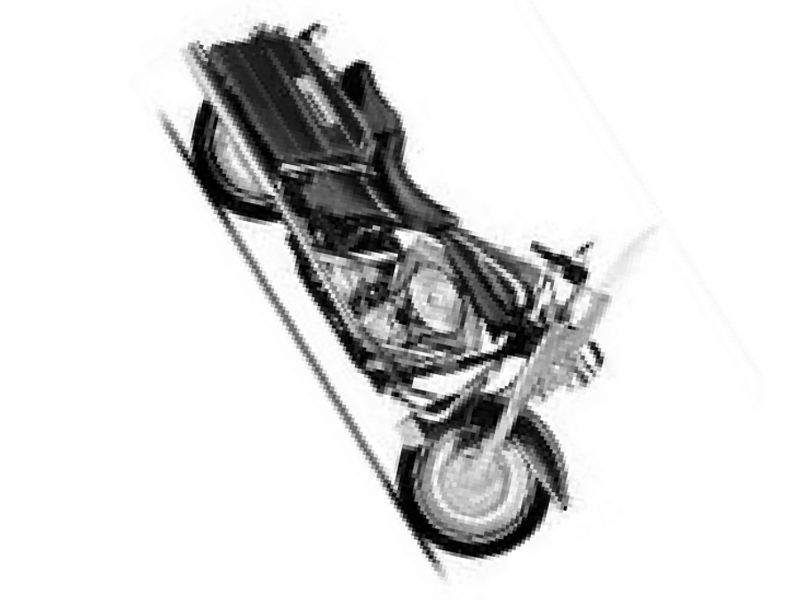
\includegraphics[width=\linewidth]{fig/reg/onebike_before2.png}
	\subcaption{Input instance}
	\label{fig/reg/concept1}
\end{subfigure}
\begin{subfigure}[b]{0.28\linewidth} \centering 
	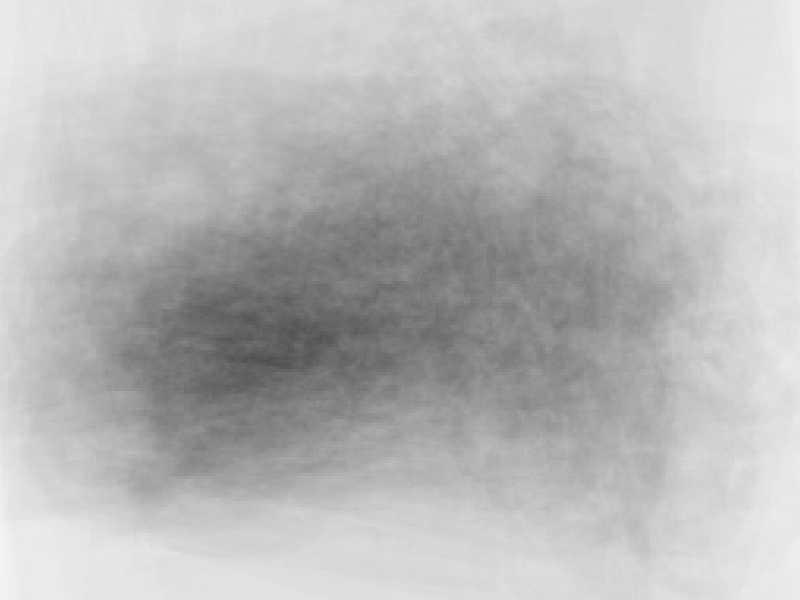
\includegraphics[width=\linewidth]{fig/reg/avgbike_before.png}
	\subcaption{Mean instance}
	\label{fig/reg/concept2}
\end{subfigure} \\ 
\begin{subfigure}[b]{0.28\linewidth} \centering
	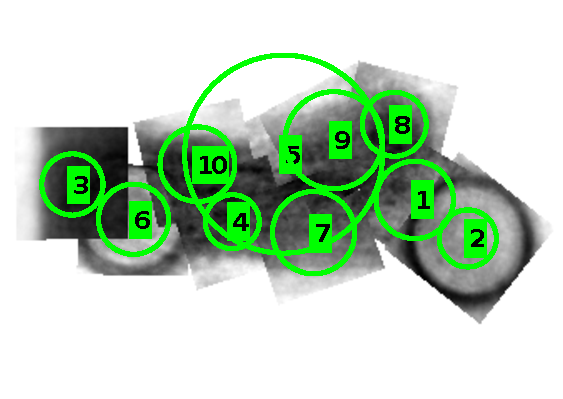
\includegraphics[width=\linewidth]{fig/reg/pictorial2.pdf}
	\subcaption{Constellation model}
	\label{fig/reg/concept4}
\end{subfigure}
\begin{subfigure}[b]{0.28\linewidth} \centering 
	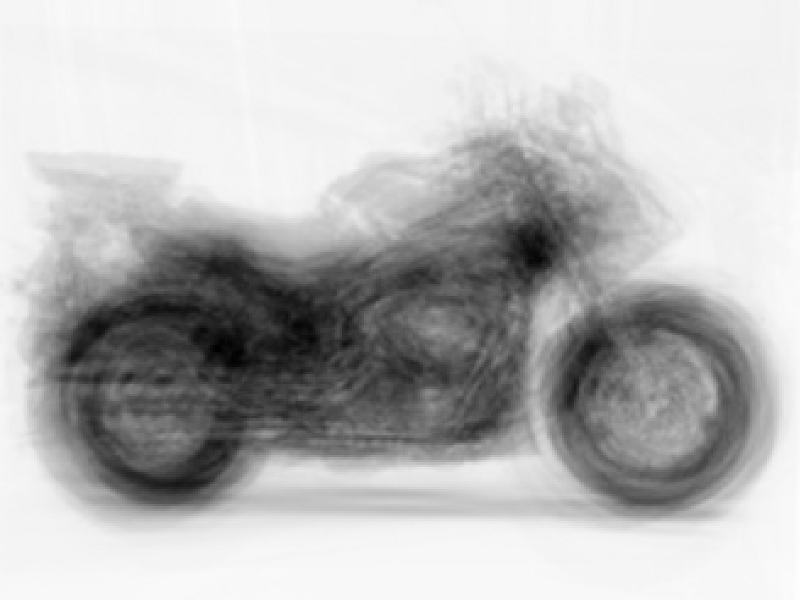
\includegraphics[width=\linewidth]{fig/reg/avgbike_after.png}
	\subcaption{Registered mean}
	\label{fig/reg/concept3}
\end{subfigure}
\begin{subfigure}[b]{0.28\linewidth} \centering 
	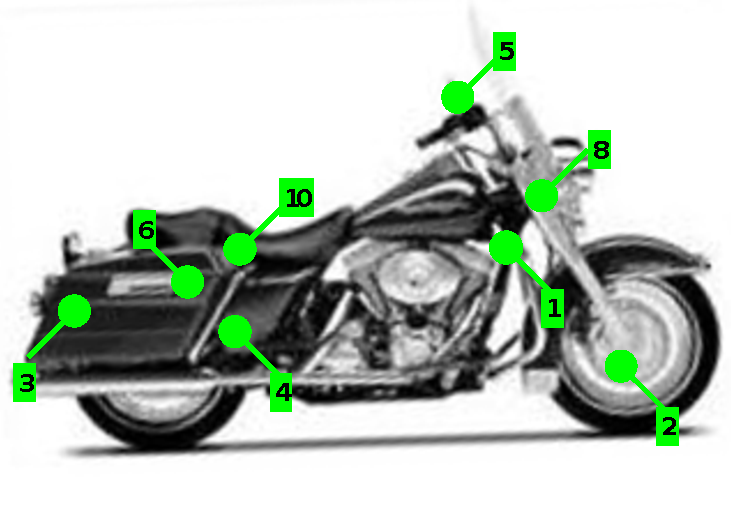
\includegraphics[width=\linewidth]{fig/reg/onebike_after3.pdf}
	\subcaption{Detected parts}
	\label{fig/reg/concept5}
\end{subfigure}
\caption{\textbf{Concept of the SAP model.} (a) A training instance, (b) mean of input instances, (c) the learned constellation model, (d) mean of registered input instances, weighted by their likelihoods, and (e) a registered instance with detected parts annotated.}
\label{fig/reg/concept}
\end{figure}

The technical contributions of the SAP model are twofold. 
This work firstly introduces a weakly-supervised learning algorithm to include instance pose as a variable in a generative probabilistic model. Additionally, the proposed particle-enhanced EM algorithm is capable of solving the resulting, difficult inference problem in both training and testing.  

%Part and vote-based methods have proved popular for object recognition tasks, overcoming the limitations of methods such as bag-of-words \cite{Sivic2005, Fei-Fei2005} and topic models \cite{Fergus2005}, by enforcing structural coherence within object classes.  Such existing methods, however, require pose information for learning.  Specifically, training data have to be aligned to a common reference frame a priori. Since modelling pose dramatically increases the dimensionality of the parameter space and hence inference complexity, this requirement precludes the use of internet-scale training datasets, \eg ImageNet \cite{Deng2009} and Tiny Image Dataset \cite{Torralba2008}, which are not generally annotated.

% Traditional computer vision tasks are usually approached by learning low level statistics on local, appearance based features, \eg bag of words \cite{Sivic2005, Fei-Fei2005} and topic models \cite{Fergus2005}, bypassing the high level structural information. These methods become less reliable in more challenging tasks, such as 3D shape recognition, when objects' textures are absent or weak in discriminative power. Making use of the spatial relationships among local features, part based model emerges as an effective solution for learning the geometric structure of an object class. Nevertheless, existing part based models require \emph{a priori pose information} for learning the structure of an object class---training data have to be registered to a common reference frame, involving extra manual processing when the poses of training or testing data are unknown. 




\section{Related work}
\label{sec/reg/relatedwork}

%%%%%%%%%%%%%%%%%%%%%%%%%%%%%%%%%%%%%%%%%%%%%%%%%%%%%%%%%%%%%%%%%%%%%%%%%%%%%%%%%%%%%%%%%%%%%%%%%
% fine
%%%%%%%%%%%%%%%%%%%%%%%%%%%%%%%%%%%%%%%%%%%%%%%%%%%%%%%%%%%%%%%%%%%%%%%%%%%%%%%%%%%%%%%%%%%%%%%%%
Local feature-based methods are widely used in object recognition tasks, thanks to their robustness to occlusion and translation. While some approaches, such as bag-of-words \cite{Sivic2005, Fei-Fei2005} and topic models \cite{Fergus2005}, use only the categorical distribution of appearance features. 

On the other side, part-based models were first articulated by Fischler and Elschlager \cite{Fischler1973} and Marr \cite{Marr1982} as a collection of movable templates or shape primitives, defined within a reference object frame. Notable part-based models include constellations \cite{Weber2000, Fergus2007} and pictorial structures (or deformable part models) \cite{Felzenszwalb2005}. Geometric structure (shape) of an object is either explained probabilistically by a model with fixed part positions \cite{Fergus2007}, or discriminatively by movable parts \cite{Yuille1989, Felzenszwalb2005}.

Early implementations of part-based models were class-specific, where parts arrangements and connections are defined before training, \eg Yuille \etal \cite{Yuille1989} detected facial features using deformable templates. While some part models remain class-specific for deformable pose estimation, \eg human poses \cite{Yang2011, Eichner2012}, recent constellation models have become more general. For instance, Burl \etal \cite{Burl1998} trained a constellation model from hand-picked parts which were represented by Gaussian distributions. Weber \etal \cite{Weber2000} improved the former approach by using an interest point detector \cite{Kadir2001} to learn feature words and approximating the feature-part assignment marginal. Fergus \etal \cite{Fergus2007} introduced scale-invariance to the model and learned shape and appearance models jointly. Most recently, constellation model was also applied to 3D shape recognition \cite{MuktaPrasad2011}.

Vote-based methods, \eg implicit shape model \cite{Leibe2008} and contour fragments \cite{Shotton2008a}, which differ from constellation models in that each feature vote consists of a fixed object pose and class. In vote-based methods, their internal object representation tends to be non-parametric, based on a codebook of appearance features, \eg k-means clustering. There is also no explicit model for background clutter, where false positives are discarded through a majority voting process. Such characteristics of vote-based methods allow for much faster inference at test stage. They have also been applied to both image-based \cite{Leibe2008, Shotton2008} and 3D shape classification \cite{Flitton2010,  Knopp2010, Pham2011, Barinova2010}.

Both part-based and vote-based approaches achieve better performance in classifying textureless objects, or objects with a high intra-class appearance variation, \eg cars or pedestrians, than appearance-only approaches. They leverage the spatial structure of an object class, at a cost of lower flexibility to pose changes.     

%Alternative approaches, such as part-based models (\eg constellation, pictorial structures) and vote-based approaches (\eg generalised hough transform), utilise the structural coherence of an object class, at a cost of lower flexibility to pose changes. 


%<<<<<<< HEAD
%%%%%%%%%%%%%%%%%%%%%%%%%%%%%%%%%%%%%%%%%%%%%%%%%%%%%%%%%%%%%%%%%%%%%%%%%%%%%%%%%%%%%%%%%%%%%%%%%
% What to do? learn relative poses! But how?
%%%%%%%%%%%%%%%%%%%%%%%%%%%%%%%%%%%%%%%%%%%%%%%%%%%%%%%%%%%%%%%%%%%%%%%%%%%%%%%%%%%%%%%%%%%%%%%%

%%%%%%%%%%%%%%%%%%%%%%%%%%%%%%%%%%%%%%%%%%%%%%%%%%%%%%%%%%%%%%%%%%%%%%%%%%%%%%%%%%%%%%%%%%%%%%%%%
% Why not use vote-based methods?
%%%%%%%%%%%%%%%%%%%%%%%%%%%%%%%%%%%%%%%%%%%%%%%%%%%%%%%%%%%%%%%%%%%%%%%%%%%%%%%%%%%%%%%%%%%%%%%%%

Although part-based and vote-based methods can be used to infer pose at test, they all require registered training instances for learning.  
Registration can be estimated from matching local features in a pre-processing step, using ICP \cite{Pham2011}, RANSAC \cite{Moreels2007}, bunch graph matching \cite{Wiskott1997} and matrix factorisation \cite{Arie-Nachimson2009}, but these require either good initialisations or manual annotations for bootstrapping. Alternatively, Learned-Miller \cite{Learned-Miller2006} proposed a data-driven method for registering an image collection.  
% However, we know of no methods which learn a shape and appearance model and infer pose of training instances \emph{jointly}.

\section{Model}
\label{sec/reg/framework}

The proposed SAP model is explained in this section. 
Firstly, given a training dataset of a particular class label, a constellation model is learned for that object class without any pose information. Pose of each training instance is initially unknown, \ie an object of that class exists somewhere in the data, which is recovered during the learning process.
Secondly, given a testing instance of unknown class, the proposed SAP model is able to estimate the class label and pose of the object in the data automatically. 

\begin{figure}[ht]
\centering
\begin{subfigure}[t]{0.48\linewidth}
	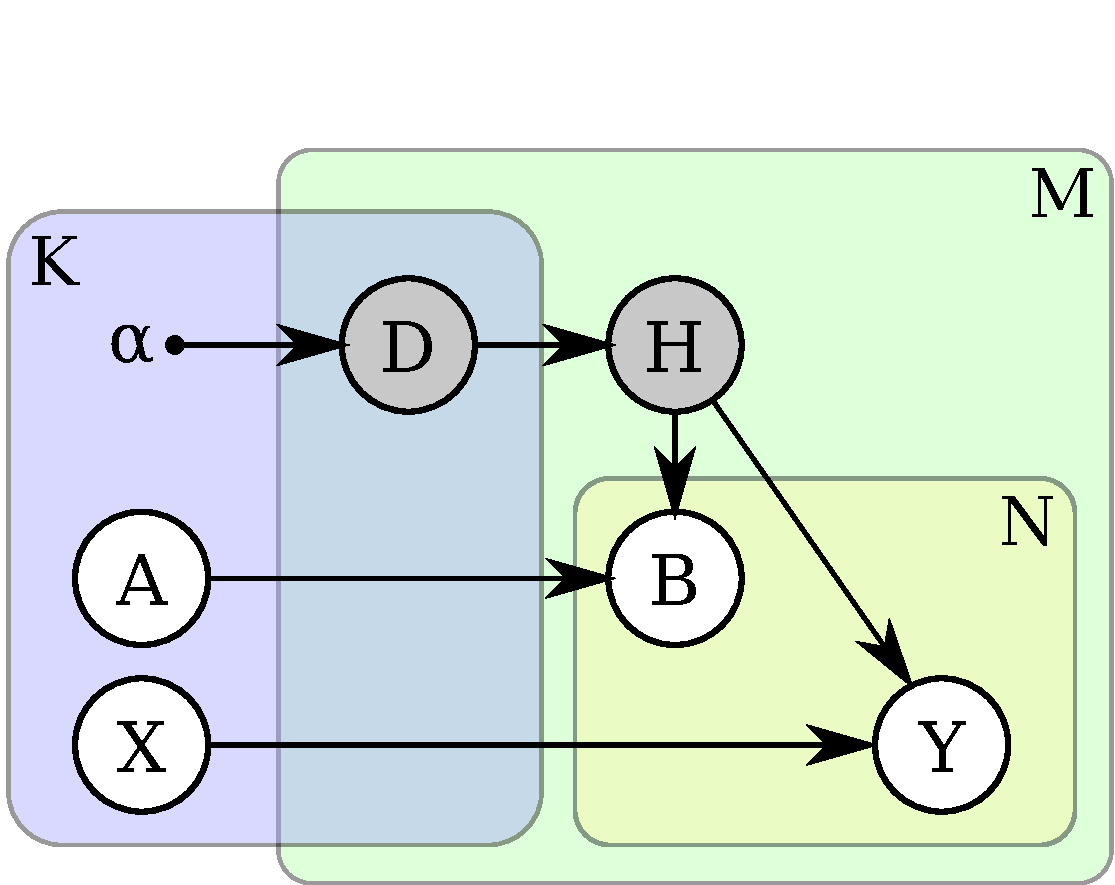
\includegraphics[width=0.8\linewidth]{fig/reg/graphicalModelNoPose.pdf}
	\subcaption{Traditional constellation model}	
	\label{fig/reg/graphicalModelNoPose}
\end{subfigure}  
\begin{subfigure}[t]{0.48\linewidth}
	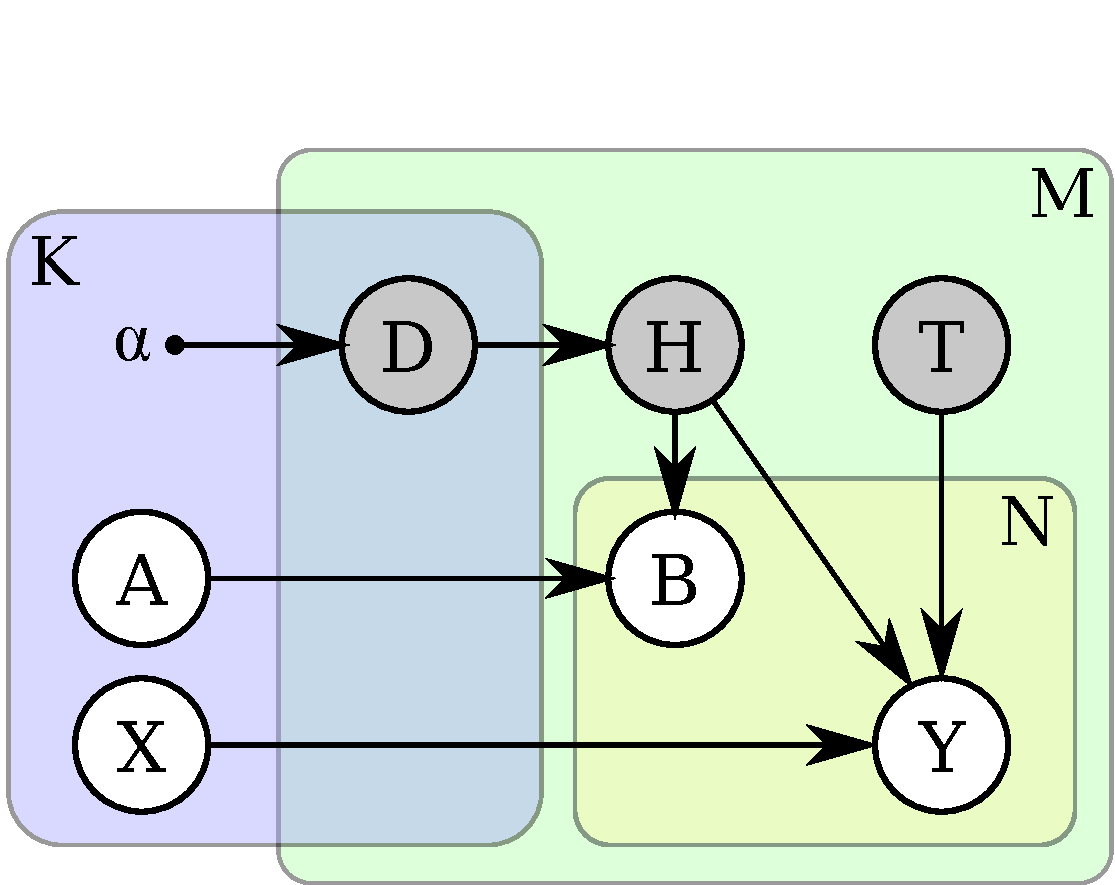
\includegraphics[width=0.8\linewidth]{fig/reg/graphicalModelNoParticle.pdf}
	\subcaption{SAP model}	
	\label{fig/reg/graphicalModelNoParticle}
\end{subfigure}
\begin{subfigure}[t]{0.48\linewidth}
	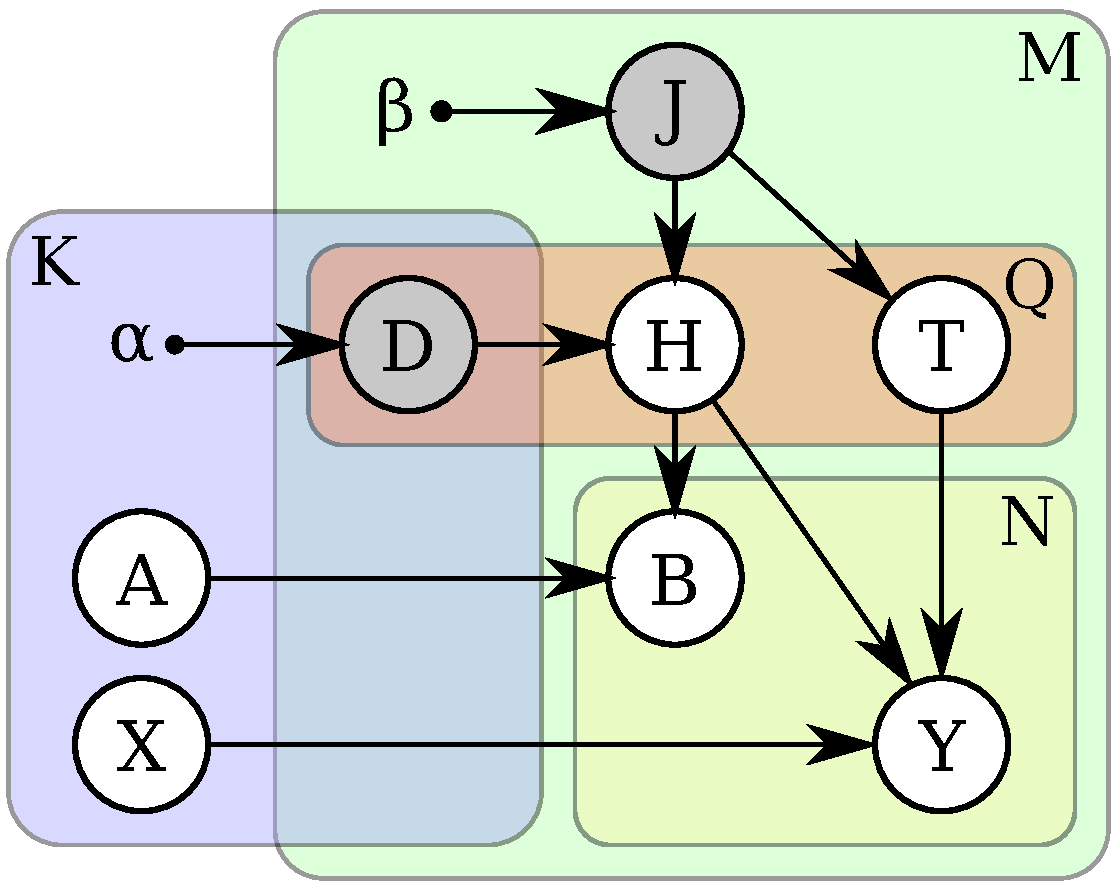
\includegraphics[width=0.8\linewidth]{fig/reg/graphicalModelParticle.pdf}
	\subcaption{SAP with particle approximation}
	\label{fig/reg/graphicalModelParticle}
\end{subfigure}
\caption{\textbf{Graphical models.} (a) Traditional constellation model, (b) SAP model without particle (c) SAP model with particles to improve inference tractability; latent variables are represented by grey nodes.}
\label{fig/reg/graphicalmodel}
\end{figure} 

\subsection{Variables}

A constellation model for a given object class is a generative model of the appearance and shape of that class, consisting of $\numpart$ object parts, each with an independent model for appearance and position in a reference frame. Appearance and position of a part are described by two Gaussians with diagonal covariances. Part appearance is represented by variable $\partapp=\{\muapp,\sigmaapp\}$, where $\muapp$ and $\sigmaapp$ are the mean and covariance of the corresponding Gaussian. Similarly, variable $\partshape=\{\mushape,\sigmashape\}$ denotes the location of a part. 

In the SAP model, each part is either visible or occluded in a given data instance.   
For simplicity, the presence of each part is independent of other parts, in contrast to \cite{Fergus2007, Weber2000}, whose model consider correlations in part occlusion. 
The visibility of a part is indicated by the binary variable, $\seen$, which equals to $1$ if the part is seen. Similar to Fergus \etal \cite{Fergus2007}, $\numfeat$ features with pose $\featshape$ and appearance $\featapp$ are identified from each data instance. (The number of extracted features, $\numfeat$, actually varies across instance. It is shown as a constant for simplicity of exposition.)  

The SAP model assumes that each feature is generated either by a part of the object, or from an unknown background class, which is represented by a part with Gaussian appearance $\{\muapp_0, \sigmaapp_0\}$ and $\{\mushape_0, \sigmashape_0\}$ respectively. 
The feature to part assignment is indicated by an variable $\assign$, which is a $\numfeat \times (\numpart + 1)$ binary indicator matrix. 
At most one feature can be assigned to an object part, whilst any number of features can be assigned to the background class, so that $\assign$ fulfils the constraints: 
\begin{equation}
	\begin{aligned}
		\sum_{\anypart = 0}^{\numpart}\assignval_{\anyfeat\anypart}& =1 & \forall \anyfeat \in [1, \numfeat], \\ 
		\sum_{\anyfeat = 1}^{\numfeat}\assignval_{\anyfeat\anypart}& =\seen_\anypart & \forall \anypart>0.
	\end{aligned} 
\end{equation}
Since $\assign$ determines the value of $\seen$, the latter appear only for convenience, and are omitted where superfluous. 

Different from other existing constellation models, object poses are explicitly modelled in learning. Each foreground object has a variable pose, $\pose$, completing the graphical model shown in figure \ref{fig/reg/graphicalModelNoParticle}, which assumes there are $\numinstance$ training/test instances. 

The appearance vectors $\partapp$ and $\featapp$ are parameterised according to the choice of feature descriptor, which is application dependent. The parameterisations of object and feature poses, which are also application dependent, have a large bearing on the tractability of the resulting inference problems, and are discussed in more detail in section \ref{sec/reg/optimisation}. 

% Each part may or may not be seen in a given data instance, independently of other parts,  \footnote{For simplicity, we assume independence of the presence of each part, in contrast to \cite{Fergus2007,Weber2000}, whose models are able to model correlations in part occlusion.} as indicated by the binary variable, $\seen$ ($=1$ if the part is seen). 
% Following Fergus \etal \cite{Fergus2007}, we extract $\numfeat$ features\footnote{The number of extracted features, $\numfeat$, varies across instances; it is constant here for simplicity of exposition.} with pose $\featshape$ and appearance $\featapp$ from each data instance; 
%the model assumes that each feature is generated either by a part from the object, or from an unknown background class (a single part with Gaussian appearance and pose distributions of $\{\muapp_0,\sigmaapp_0\}$ and $\{\mushape_0,\sigmashape_0\}$ respectively), according to an assignment, $\assign$. 
%\footnote{Since $\assign$ determines the $\seen$ values, the latter appear only for convenience, and are omitted where superfluous.} In addition, we novelly assume that the foreground object itself has a variable pose, $\pose$, completing the graphical model shown in figure \ref{fig/reg/graphicalModelNoParticle}, which assumes there are $\numinstance$ training/test instances.


\paragraph{Notation~} Many of the random variables in the proposed model are one of an independent set, indicated by the plates (boxes) in figure \ref{fig/reg/graphicalmodel}. The variable sets using the same letters in calligraphic font, while variables are indexed within these sets by subscript lowercase letters matching the uppercase letter indicating the number of elements in the set. For example, the set of part-feature assignments over all instances is $\setassign = \{\assign_{\anyinstance}\}_{\anyinstance=1}^\numinstance$. Set and subset indices are concatenated, \eg $\assignval_{\anyinstance\anyfeat\anypart}$.

\subsection{Distributions}

Distributions of the proposed SAP model are parameterised as follows. Firstly, the visibility of a part $\anypart$ is formulated as:
\begin{align}
	\prob(\seen_{\anypart}) = & \partprior_\anypart^{\seen_{\anypart}}\cdot(1-\partprior_\anypart)^{1-\seen_{\anypart}} \partprior_\anypart\in[0, 1], 
	\label{eqn/reg/Ddist}
\end{align}
where $\partprior_\anypart\in [0, 1]$ is a binomial prior of a single part. Given a list of visible part $\seen$, the probability of assignment $\prob(\assign|\setseen)$ is 
\begin{align}
	\prob(\assign|\setseen) = & 
	\begin{cases} 
		\displaystyle\frac{(\numfeat - \displaystyle\sum_{\anypart=1}^{\numpart}\seen_\anypart)!}{\numfeat!} & \mbox{ if } \seen_\anypart = \displaystyle\sum_{\anyfeat=1}^{\numfeat}\assignval_{\anyfeat\anypart},   \forall\anypart\in\{1,..,\numpart\} \\[3mm]
	0 & \mbox{otherwise} 
	\end{cases},
	\label{eqn/reg/HDdist}
\end{align}
where all valid assignments forms a uniform distribution. The distribution of observed appearance $\featapp$ given $\setpartapp$ and $\assign$ is modelled as a joint normal distribution of all visible parts:  
\begin{equation}
	\prob(\featapp|\setpartapp,\assign) = \displaystyle\prod_{\anypart=0}^\numpart
	\NormDist(\featapp; \muapp_\anypart, \sigmaapp_\anypart)^{\assignval_{\anyfeat\anypart}}.
	\label{eqn/reg/appearance}
\end{equation}
Similarly, the probability of observed spatial arrangement, given model shape $\setpartshape$, assignment $\assign$ and object pose $\pose$, is defined as 
\begin{align}
	\displaystyle\prob(\featshape|\setpartshape,\assign,\pose) = & \prod_{\anypart=0}^\numpart
	\left[\frac{\textstyle\exp\left(-\dist(\pose\comp\featshape, \mushape_\anypart; \sigmashape_\anypart)^2\right)}{\displaystyle\int_{\mathbf{Z}} \exp\left(-\dist(\mathbf{Z}, \mushape_\anypart; \sigmashape_\anypart)^2\right)}\right]^{\assignval_{\anyfeat\anypart}}.
	\label{eqn/reg/shape}
\end{align}
The above distribution is in the non-Euclidean shape space, characterised by the distance function, $\dist()$. Object pose $\pose$ is assumed to be a linear, where feature shapes $\featshape$ are transformed by multiplying with the pose matrix $\pose$.   

\section{Learning}
The learning algorithm seek to maximise the posterior probability of the constellation model parameters, $\setpartapp$ and $\setpartshape$, with respect to the $\numinstance$ given instances:  
\begin{equation}
	\begin{aligned}
		\setpartapp,\setpartshape & = \argmax_{\setpartapp, \setpartshape}
		\prob(\setpartapp,\setpartshape)
		\prod_{\anyinstance=1}^\numinstance 
		\frac{\prob(\setfeatapp_\anyinstance,\setfeatshape_\anyinstance|\setpartapp,\setpartshape)}{\prob(\setfeatapp_\anyinstance,\setfeatshape_\anyinstance)} \\ 
		& = \argmax_{\setpartapp, \setpartshape}
		\prod_{\anyinstance=1}^\numinstance 
		\prob(\setfeatapp_\anyinstance,\setfeatshape_\anyinstance|\setpartapp,\setpartshape).
	\end{aligned}
\end{equation}
Assuming a uniform $\prob(\setpartapp,\setpartshape)$, the objective is equivalent to maximising their likelihood, since $\prob(\setfeatapp_\anyinstance,\setfeatshape_\anyinstance)$ is constant.  
Normally $\prob(\setfeatapp_\anyinstance, \setfeatshape_\anyinstance | \setpartapp, \setpartshape)$ is computed by marginalising over $\assign$ and $\pose$, which in this scenario are both latent variables, thus:
\begin{equation}
	\prob(\setfeatapp_\anyinstance,\setfeatshape_\anyinstance|\setpartapp,\setpartshape) = 
	\sum_{\assign_\anyinstance \in \allassign}
	\displaystyle\int_{\pose_\anyinstance}
	\prob(\setfeatapp_\anyinstance,\setfeatshape_\anyinstance,\assign_\anyinstance,\pose_\anyinstance|\setpartapp,\setpartshape).
	\label{eqn/reg/learningobjective}
\end{equation}
However, given that the number of possible assignments, $|\allassign|$, is exponential in both $\numpart$ and $\numfeat$, whilst the instance pose, $\pose$, is a multi-dimensional, continuous variable in a non-Euclidean space, both the integrations are practically intractable. For this reason, a particle-based algorithm is employed to approximate the solution without computing all possible assignments and poses.  

% two definition here 
\def\spfparticlem{\particle_{\anyinstance}  =  \anyparticle}
\def\spfparticle{\particle  =  \anyparticle} 
\subsection{Particle-based approximation}

It is assumed that the vast majority of the mass in the distribution occurs around the optimal configuration of pose and feature assignment for each instance. The particles can be seen as samples of the joint space of $\assign$ and $\pose$, making this technique similar to the Monte Carlo Expectation Maximisation algorithm \cite{Levine2001, Wei1990}, which uses samples to approximate integrations over latent variables. However, the proposed model aims to maximise the likelihood of particles, by optimising $\assign$ and $\pose$, rather than sampling them randomly from the distribution. 

The marginalisation in equation \ref{eqn/reg/learningobjective} can be approximated by sampling points in the solution space, such that 
\begin{equation}
	\begin{aligned}
		\setpartapp,\setpartshape = & \argmax_{\setpartapp,\,\setpartshape}
		\displaystyle\prod_{\anyinstance=1}^\numinstance
		\prob(\setfeatapp_\anyinstance,\setfeatshape_\anyinstance|\setpartapp,\setpartshape) \\ 
		\approx &  
		\argmax_{\setpartapp,\,\setpartshape}
		\displaystyle\prod_{\anyinstance=1}^\numinstance
		\max_{\assign_\anyinstance,\,\pose_\anyinstance}
		\prob(\setfeatapp_\anyinstance,\setfeatshape_\anyinstance,\assign_\anyinstance,\pose_\anyinstance|\setpartapp,\setpartshape).
	\end{aligned}
	\label{eqn/reg/approximatemaximumpose}
\end{equation}
However, it is highly unlikely that the objective function is convex, hence there exist local maxima over the solution space. A local optimisation approach, initialised na\"{i}vely, will probably converge to one of the local maxima, producing a poor solution. 
To overcome this issue, $\numparticle$ pose particles (sampling points) are created per instance, each with associated feature assignment and pose. They are then initialised randomly in order to increase the chances of finding the optimal solution. 
Consequently, the particles are represented by a new latent variable $\particle$ in the proposed model, which indicates the index of pose particle that represents the correct pose. This leads to the graphical model shown in figure \ref{fig/reg/graphicalModelParticle}. Marginalising over the $\numparticle$ possible values of $\particle$ per instance, given that 
$\prob(\pose_{\anyinstance\anyparticle}|\particle_{\anyinstance}  =  r)$ and $\prob(\assign_{\anyinstance\anyparticle}|\particle_{\anyinstance}  =  r)$ are delta distributions at $\anyparticle=r$, the final training objective function is: 
\begin{equation}
	\setpartapp,\setpartshape = \argmax_{\setpartapp,\,\setpartshape}
	\prod_{\anyinstance=1}^\numinstance \sum_{\anyparticle = 1}^{\numparticle} 
	\prob(\spfparticlem)
	\max_{\assign_{\anyinstance\anyparticle},\,\pose_{\anyinstance\anyparticle}} \prob(\setfeatapp_\anyinstance,\setfeatshape_\anyinstance,\assign_{\anyinstance\anyparticle},\pose_{\anyinstance\anyparticle}|\setpartapp,\setpartshape), 
	\label{eqn/reg/particleapproximation}
\end{equation}
\begin{equation}
	\begin{aligned}
	& \prob(\setfeatapp,\setfeatshape,\assign,\pose|\setpartapp,\setpartshape) \\  
	= & \prod_{\anyfeat=1}^\numfeat
	\prob(\featapp_{\anyfeat}|\setpartapp,\assign)
	\prob(\featshape_{\anyfeat}|\setpartshape,\assign,\pose)
	\sum_{\setseen}
	\prob(\assign|\setseen)
	\prod_{\anypart=1}^\numpart
	\prob(\seen_{\anypart}),
	\end{aligned}
	\label{eqn/reg/decompose}
\end{equation}
according to the decomposition specified by the model in figure \ref{fig/reg/graphicalModelParticle}.
Note that the marginalisation over $\setseen$ is trivial since equation \ref{eqn/reg/HDdist} implies that, given $\assign$, only one value is possible. 
The probability of observing the $\particle$-th particle $\prob(\particle)$ is a categorical distribution:
\begin{equation}
	\begin{aligned}
		\prob(\spfparticle) & = \particleprior_\anyparticle, & ~ \mbox{ where }   \sum_{\anyparticle=1}^\numparticle \particleprior_\anyparticle = 1. 
	\end{aligned}
\end{equation}

\section{Testing}

Given the object class parameters obtained from training, $\setpartapp$ and $\setpartshape$, the proposed SAP constellation model determines whether an object is present in the data. Meanwhile, it also estimates the most probable pose of the object. 
The posterior probability of a given class being present is given by equation \ref{eqn/reg/testposterior}: 
\begin{equation}
	\prob(\fg|\setfeatapp,\setfeatshape) = \displaystyle\frac{\prob(\fg)}{\prob(\setfeatapp,\setfeatshape)}\max_{\pose}\sum_{\assign \in \allassign}\prob(\setfeatapp,\setfeatshape,\assign,\pose|\setpartapp,\setpartshape).
	\label{eqn/reg/testposterior}
\end{equation}
However, as previously mentioned, marginalisation of $\assign$ is avoided using the same particle-based approximation as in training:
\begin{equation}
	\prob(\fg|\setfeatapp,\setfeatshape) \approx \displaystyle\frac{\prob(\fg)}{\prob(\setfeatapp,\setfeatshape)} \sum_{\anyparticle=1}^\numparticle \prob(\spfparticle)
	\max_{\pose_\anyparticle,\,\assign_\anyparticle} \prob(\setfeatapp,\setfeatshape,\assign_\anyparticle,\pose_\anyparticle|\setpartapp,\setpartshape).
	\label{eqn/reg/testobjective}
\end{equation}
Similarly, the expression is then decomposed according to equation \ref{eqn/reg/decompose}.
The object pose is then computed by finding the value of $\pose_\anyparticle$ for the most likely particle, \ie for which $\prob(\spfparticle)$ is largest.

This probability can then be used in binary or multi-class object classifiers by comparing the probabilities given for different object classes, including the background class, \ie no object is present in the data. The value $\prob(\setfeatapp,\setfeatshape)$ is constant across classes thus it can be ignored. The a priori class distribution, $\prob(\fg)$, can be given or learned. For simplicity, this work assumes an uniform class prior. 

\section{Inference}
\label{sec/reg/optimisation}

Since both training and test objective functions, given by equations \ref{eqn/reg/particleapproximation} and \ref{eqn/reg/testobjective} respectively, involve the latent $\particle$ variables, expectation maximisation (EM) algorithm can be used for inference. 
Given the likelihood of model parameters in the previous iteration $\parameter^{(t-1)} = \{\partprior^{(t-1)},\particleprior^{(t-1)},\assign^{(t-1)},\setpartapp^{(t-1)},\pose^{(t-1)},\setpartshape^{(t)}\}$ is defined as
\begin{equation}
	\expect = \frac{\prob(\spfparticlem)\prob(\setfeatapp_\anyinstance,\setfeatshape_\anyinstance,\assign^{(t-1)}_{\anyinstance\anyparticle},\pose^{(t-1)}_{\anyinstance\anyparticle}|\setpartapp^{(t-1)},\setpartshape^{(t-1)})}{\displaystyle\sum_{\anotherparticle = 1}^{\numparticle} \prob(\particle_{\anyinstance}  =  \anotherparticle)\prob(\setfeatapp_\anyinstance,\setfeatshape_\anyinstance,\assign^{(t-1)}_{\anyinstance\anotherparticle},\pose^{(t-1)}_{\anyinstance\anotherparticle}|\setpartapp^{(t-1)},\setpartshape^{(t-1)})}.
\end{equation}
Current parameter estimates $\parameter^{(t)}$ is estimated by maximising the above likelihood. To this end, an auxiliary function $\EMQ$ is actually maximised in the maximisation-step (M-step):  
\begin{equation}
	\EMQ = \displaystyle\sum_{\anyinstance=1}^\numinstance \displaystyle\sum_{\anyparticle = 1}^{\numparticle} \expect \log \left( \prob(\spfparticlem)\prob(\setfeatapp_\anyinstance,\setfeatshape_\anyinstance,\assign^{(t)}_{\anyinstance\anyparticle},\pose^{(t)}_{\anyinstance\anyparticle}|\setpartapp^{(t)},\setpartshape^{(t)}) \right).
	\label{eqn/reg/auxiliary}
\end{equation}
The updates for the M-step are obtained by setting the derivative of the auxiliary function $\EMQ$ with respect to each target parameter to zero. Since the parameters are interdependent, but optimised separately, this part of the algorithm effectively consists of an iteration of coordinate descent. The computations required for each step are described below.

Part appearances and shapes $\setpartapp$ and $\setpartshape$ are updated during training, but these variables are fixed during testing. Besides this, the two optimisation algorithms are identical. 

\begin{algorithm} 
	\begin{algorithmic}
		\STATE Initialise $\parameter^{(0)}$.
		\REPEAT
		\STATE \textbf{E-step} (expectation step): 
		\STATE \hspace{\algorithmicindent} Evaluate the latent likelihood $\expect$ from $\parameter^{(t-1)}$.   
		\STATE \textbf{M-step} (maximisation step): 
		\STATE \hspace{\algorithmicindent} Maximise $\EMQ$ w.r.t. part prior $\partprior^{(t)}$
		\STATE \hspace{\algorithmicindent} Maximise $\EMQ$ w.r.t. particle prior $\particleprior^{(t)}$
		\STATE \hspace{\algorithmicindent} Maximise $\EMQ$ w.r.t. assignment $\assign^{(t)}$
		\STATE \hspace{\algorithmicindent} In training, maximise part appearance $\EMQ$ w.r.t. $\partapp^{(t)}$ 
		\STATE \hspace{\algorithmicindent} Maximise $\EMQ$ w.r.t. object pose $\pose^{(t)}$
		\STATE \hspace{\algorithmicindent} In training, maximise $\EMQ$ w.r.t. part shape $\partshape^{(t)}$
		\UNTIL{Likelihood $\expect$ converges}
	\end{algorithmic}
	\caption{\textbf{Overview of the EM algorithm.}}
	\label{algo/reg/em}
\end{algorithm} 

\subsection{Learning model parameters} 

\subsubsection{Updating $\partprior$, $\particleprior$}  The update equations are

\begin{equation}
	\partprior_{\anypart} = \frac{\displaystyle\sum_{\anyinstance=1}^\numinstance \sum_{\anyparticle = 1}^{\numparticle} \expect\seen_{\anyinstance\anyparticle\anypart}}{\displaystyle\sum_{\anyinstance=1}^\numinstance \sum_{\anyparticle = 1}^{\numparticle} \expect}, 
\end{equation}

\begin{equation}
\particleprior_{\anyinstance\anyparticle} = 
\frac{\expect}{\displaystyle\sum_{\anyparticle = 1}^{\numparticle} \expect}.
\end{equation}

\subsubsection{Updating $\assign$}
Taking negative logs of the terms in equation \ref{eqn/reg/decompose} leads to a sum of costs to be minimised, all of which are linear in $\assign$, except for $-\log\prob(\assign|\setseen)$. 
However, since generally only a small portion of features are actually assigned to parts, \ie $\sum_{\anypart=1}^{\numpart}\seen_\anypart \ll \numfeat$, then $-\log\prob(\assign|\setseen)$ is linearly approximated by $\sum_{\anypart=1}^{\numpart}\seen_\anypart\log\numfeat$,  as $\seen_\anypart$ being a linear function of $\assign$. The optimal $\assign$ for this approximate cost function $\order\left((N + K)^3\right)$ is computed using a linear assignment solver such as the Hungarian algorithm.  

\subsubsection{Updating $\setpartapp$}
The part appearances, $\partapp_\anypart$, are updated by computing a weighted mean and variance of the feature appearances, $\featapp_{\anyinstance\anyfeat}$. A weight function is first defined in equation \ref{eqn/reg/weightedavg}:
\begin{equation}
	\wavg_k(x) = \frac{\displaystyle\sum_{\anyinstance=1}^\numinstance \displaystyle\sum_{\anyparticle = 1}^{\numparticle} \displaystyle\sum_{\anyfeat=1}^{\numfeat}\expect\assignval_{\anyinstance\anyfeat\anyparticle\anypart} \cdot x}{\displaystyle\sum_{\anyinstance=1}^\numinstance \displaystyle\sum_{\anyparticle = 1}^{\numparticle} \displaystyle\sum_{\anyfeat=1}^{\numfeat}\expect\assignval_{\anyinstance\anyfeat\anyparticle\anypart}}.
	\label{eqn/reg/weightedavg} 
\end{equation}
The part appearance, represented by mean $\muapp_{\anypart}^{(t)}$ and covariance $\sigmaapp_{\anypart}^{(t)}$, is updated as follows:  
\begin{equation}
	\begin{aligned}
		\muapp_{\anypart}^{(t)} & = \wavg_k(\featapp_{\anyinstance\anyfeat}), \\[3mm]  
		\sigmaapp_{\anypart}^{(t)} & = \wavg_k((\featapp_{\anyinstance\anyfeat} - \muapp_{\anypart}^{(t)})(\featapp_{\anyinstance\anyfeat} - \muapp_{\anypart}^{(t)})^\trsp).
	\end{aligned}
	\label{eqn/reg/partappearance}
\end{equation}
Since the weights in equation \ref{eqn/reg/partappearance} depend on other part appearances, the optimal $\setpartapp$ is not maximised in a single iteration. Nevertheless, the equation approaches to the optimal solutions when the M-step are iterated. 

\subsubsection{Updating $\pose$}
The instance pose, $\pose$, can be parameterised in various ways, depending on the pose variations seen in the data. In this work two different parameterisations are considered. The first is the direct similarity transform
\begin{equation}
	\pose=\left[\begin{array}{cc}
			s(\pose)\mathbf{R}(\pose) & \mathbf{t}(\pose)\\
		\mathbf{0}^\trsp & 1\end{array}\right],
	\label{eqn/reg/dsmatrix}
\end{equation}
where $s(\pose)\in\mathbb{R}^+$, $\mathbf{R}(\pose)\in SO(l,\mathbb{R})$, and $\mathbf{t}(\pose)\in\mathbb{R}^l$ are the scale, rotation, and translation components respectively; and $l$ is the dimensionality of input data. 

In this case the part/feature positions, $\partshape$ and $\featshape$, adopt the SRT distance \cite{Pham2011} for the distance function $d()$ in equation \ref{eqn/reg/shape}. In the SRT distance, a feature is represented by a similarity transformation matrix, similar to \ref{eqn/reg/dsmatrix}. The weighting for scale, rotation and translation in SRT distance are denoted by parameters $\sigmashape = \{\sigmashapes, \sigmashaper, \sigmashapet\}$.
According to Pham \etal \cite{Pham2011}, the SRT distance has the desirable properties of a closed form weighted mean and a constant Gaussian normalisation factor. This not only eliminates scale bias, but also introduces feature orientation into the constellation model.

The second is the affine transform, represented by a matrix similar to that above, but whose first $l$ rows can take any real values. In this situation the part/feature positions are parameterised by translation only, and $d()$ is simply Euclidean distance.

The update steps for object pose are summarised as below. 
For the direct similarity transform, $\EMQ$ is differentiated w.r.t. each of the pose parameters in the order $\mathbf{t}(\pose)$ (translation), $\mathbf{R}(\pose)$ (rotation), $s(\pose)$ (scale), and set to zero. For the first two components this yields a closed form update, while $s(\pose)$ is computed using Newton-Raphson. 
%For the affine transform, setting the derivative to zero leads to a closed form update.

Since the pose parameters are interdependent, this update is not optimal, but it does increase the model probability.
A degenerate case is where the pose scale component, $s(\pose)$, of any instance particle becomes zero. This issue is addressed by normalising the weighted average pose scale to one at the end of each M-step. Since the SRT distance used in equation \ref{eqn/reg/shape} is scale-invariant \cite{Pham2011}, this does not alter the model probability distribution. Such pose normalisation changes the likelihood for the affine SAP model, however, the decrease in likelihood is approximately constant so it can be estimated without affecting the EM algorithm.

\subsubsection{Updating $\setpartshape$}
The mean part positions, $\mushape_\anypart$, are updated according to \cite{Pham2011}, using the same weight as in equation \ref{eqn/reg/weightedavg}. The bandwidth parameters are updated as follows:
\begin{align}
	\sigmashapet_{\anypart}^{(t)} & = \wavg_k\left((\mathbf{t}(\featapp_{\anyinstance\anyfeat}) - \mathbf{t}(\mushape_{\anypart}^{(t)}))(\mathbf{t}(\featapp_{\anyinstance\anyfeat}) - \mathbf{t}(\mushape_{\anypart}^{(t)}))^\trsp\right) \label{eqn/reg/updatemeant}, \\[3mm] 
	\sigmashaper_{\anypart}^{(t)} & = \wavg_k\left((\mathbf{R}(\featapp_{\anyinstance\anyfeat}) - \mathbf{R}(\mushape_{\anypart}^{(t)}))(\mathbf{R}(\featapp_{\anyinstance\anyfeat}) - \mathbf{R}(\mushape_{\anypart}^{(t)}))^\trsp\right) \label{eqn/reg/updatedmeanr}, \\[3mm]
	\sigmashapes_{\anypart}^{(t)} & = \wavg_k\left(\log^2\left(\frac{s(\featapp_{\anyinstance\anyfeat})}{s(\mushape_{\anypart}^{(t)})}\right)\right). \label{eqn/reg/updatemeans}
\end{align}
Since the affine poses cannot be uniquely factorised to SRT components, only the update steps for translation components, \ie $\mathbf{t}(\mushape_\anypart)$ and $\sigmashapet$, are performed for the affine pose SAP model. 

\subsubsection{Initialisation}
Initial parameters $\parameter^{(0)}$ for the EM algorithm are computed as follows. Firstly, the particle poses $\pose^{(0)}$ for each instance are each assigned the inverse pose of an instance feature selected at random. Secondly, parameters $\partprior$ and $\particleprior$ are initialised uniformly as $1/2$ and $1/\numparticle$. Thirdly, k-means clustering is performed on the feature positions $\pose^{(0)}\featshape$, and initial parts $\{\partapp^{(0)}, \partshape^{(0)}\}$ are estimated from the k-means assignments. Finally, assignments $\assign^{(0)}$ are selected by maximising the likelihood of the initial shape model.

\subsubsection{Particle considerations}
The computational cost of learning the model is linear in the number of particles, $\numparticle$, while there are diminishing returns to be had from increasing $\numparticle$, in terms of successful model convergence. The best number of particles is very much application and data dependent. In the experiments of this chapter, 5--10 particles were sufficient to produce good results, further increasing the number of particle would only accelerate convergence marginally, but computation time was increased linearly. 

By allowing every instance to have multiple poses, equivalent sub-models can form within the model.
To avoid this issue, after the first convergence, the most probable training instance (with the highest likelihood) is selected, and its most probable particle (with highest likelihood) is retained and fixed, while all other particles are removed. As a result, the pose of the selected instance will be fixed in the subsequent iterations, effectively defining the single \emph{canonical pose} of the class. 
% To avoid this, after the first convergence of EM we select the instance with the highest likelihood and remove all but one of its particles (that with the highest likelihood), whose pose we then keep fixed, essentially defining the single \emph{canonical pose} of the class.
Furthermore, when the likelihood of particles heads to zero, or two or more particles converge on the same pose, updating them becomes computationally wasteful. To avoid this, those superfluous particles can either be removed, or their poses can be re-initialised at random. This stochastic approach is applied to aid convergence to a good local optimum.  

% TODO - 
% Restructure the section: divide it by datasets not applications (reg and rec)
% Since exact ground truth is not provided 

\section{Experiments}
\label{sec/reg/experiments}


%We evaluate both registration performance (during both training and test) and recognition performance, on both 2D image data and 3D point cloud data.

The performance evaluation was divided into two parts. Experiments were performed to justify the versatility of the proposed SAP model under different types of input (2D images and 3D shapes) and applications (registration and recognition). This section details the experimental setup and reports the experimental results.

\subsection{Datasets}
% Maybe good to have a figure showing some sample data when we have enough space.
%The first part evaluated the proposed model with respect to object recognition tasks. 
%The second part investigates the pose learning capability of the proposed approach. 
%Two types of data are used in the experiments to demonstrate the flexibility of the proposed model in different potential applications. 
% The model parameters, if not learned, are listed in table \ref{tab/reg/parameters}. 
%\paragraph{Evaluation datasets} 
% 2D dataset, introduction

\begin{figure}[t]
	\centering
	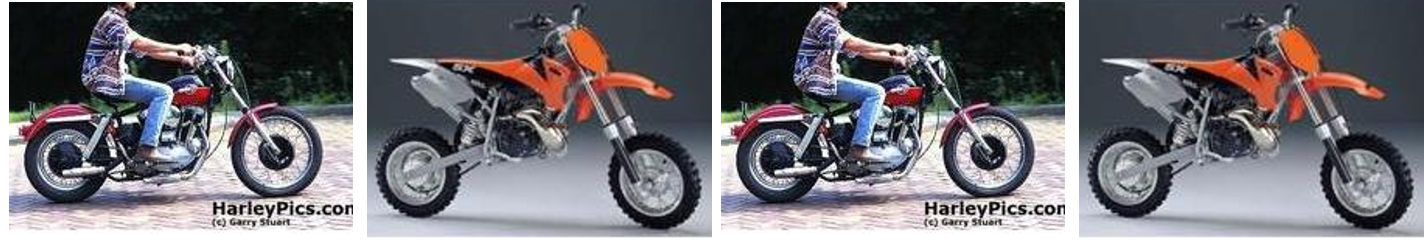
\includegraphics[width=1\linewidth]{./fig/reg/bike_long.png}
	\caption{\textbf{Sample images of the \textbf{bike} dataset.}}
	\label{fig/reg/bike}
\end{figure}

\subsubsection{2D evaluation dataset}
Experiments for 2D classification and registration was performed using the Caltech \textbf{bike} dataset \cite{ComputationalVisionLab2001}, which contains 800 generic background images and 800 motorbike images with large inter-class appearance variations, cluttered backgrounds and moderately varying poses. Figure \ref{fig/reg/bike} shows several sample images of the \textbf{bike} dataset.  
Features were detected in each image over translation and scale, using the method described in Fergus \etal \cite{Fergus2007}. 
For the \textbf{bike} dataset, feature position, $\featshape_{\anyinstance\anyfeat}$, were located using the Kadir and Brady saliency detector \cite{Kadir2001}. The SRT reference frames of detected interest points were completed by assigning an $8$-quantised principal orientation to each of them, according to the corresponding histogram of gradient. 
Rotated patches of the interest points were extracted from the images and resized to $15 \times 15$ pixels in size.
The $255$-dimensional appearance space feature was embedded to a compact $15$-dimensional space using PCA. 

%Each feature position, $\featshape_{\anyinstance\anyfeat}$, was then completed by computing an $8$-quantised principal orientation from pixel gradients of the local patch. 
%Appearance vectors, $\featapp_{\anyinstance\anyfeat}$, were computed by projecting the local patches into a compact $15$-dimensional space using PCA.  

% 3D dataset, introduction
\subsubsection{3D evaluation dataset}

\begin{figure}[t]
	\centering
	\begin{subfigure}[b]{0.16\linewidth} \centering
		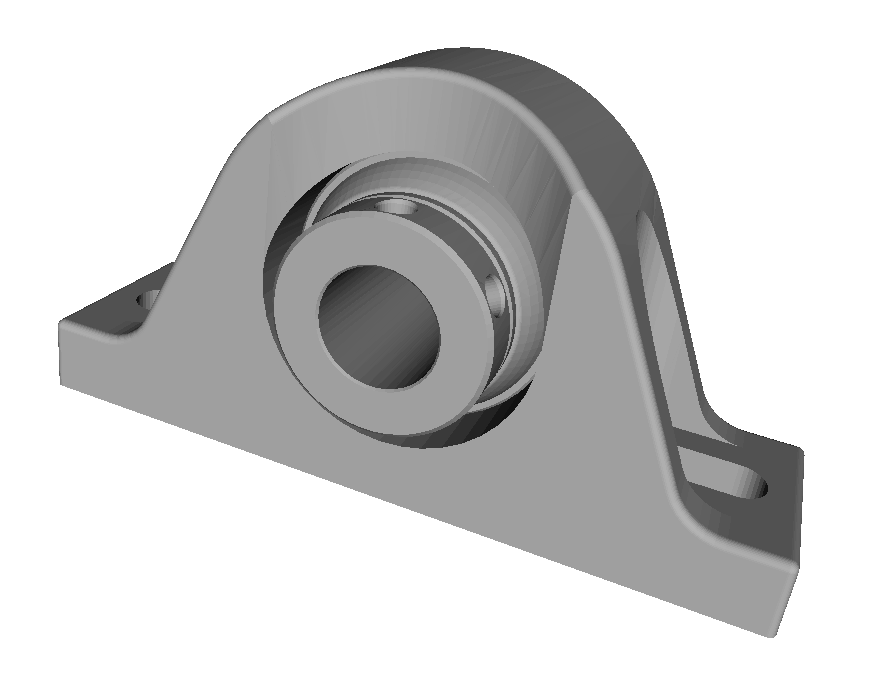
\includegraphics[width=1\linewidth]{./fig/eval/toshiba_bearing1.png}
		\caption{Bearing}
	\end{subfigure}
	\begin{subfigure}[b]{0.16\linewidth} \centering
		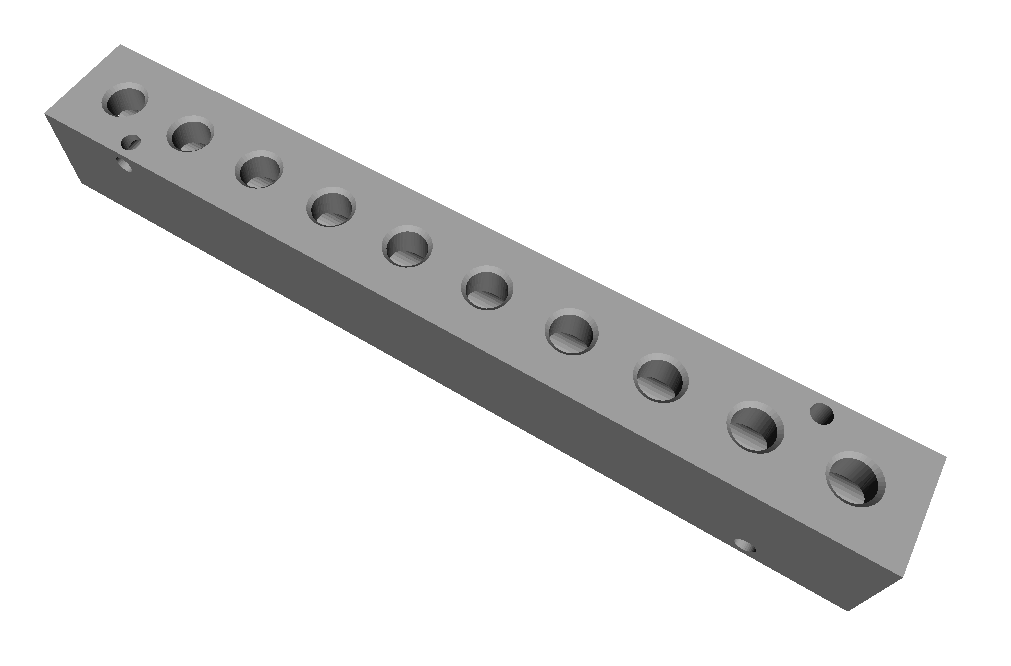
\includegraphics[width=1\linewidth]{./fig/eval/toshiba_block1.png}
		\caption{Block}
	\end{subfigure}
	\begin{subfigure}[b]{0.16\linewidth} \centering
		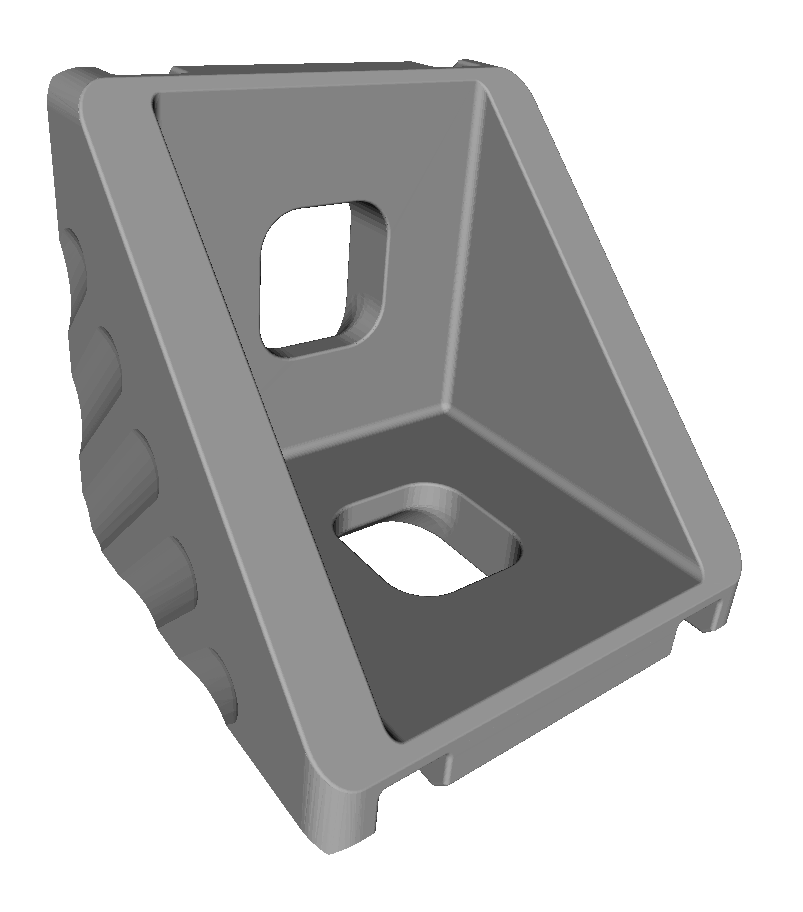
\includegraphics[width=1\linewidth]{./fig/eval/toshiba_bracket1.png}
		\caption{Bracket}
	\end{subfigure}
	\begin{subfigure}[b]{0.16\linewidth} \centering
		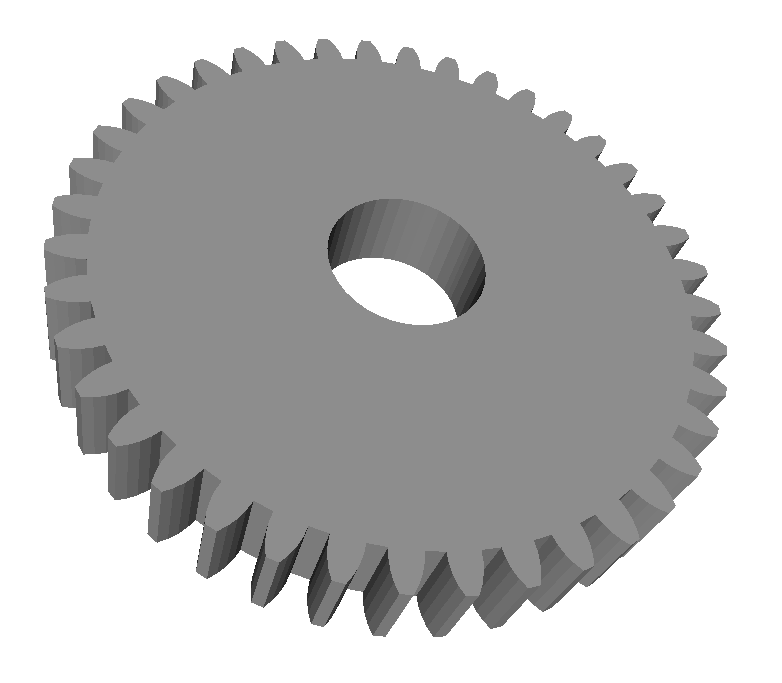
\includegraphics[width=1\linewidth]{./fig/eval/toshiba_cog1.png}
		\caption{Cog}
	\end{subfigure}
	\begin{subfigure}[b]{0.16\linewidth} \centering
		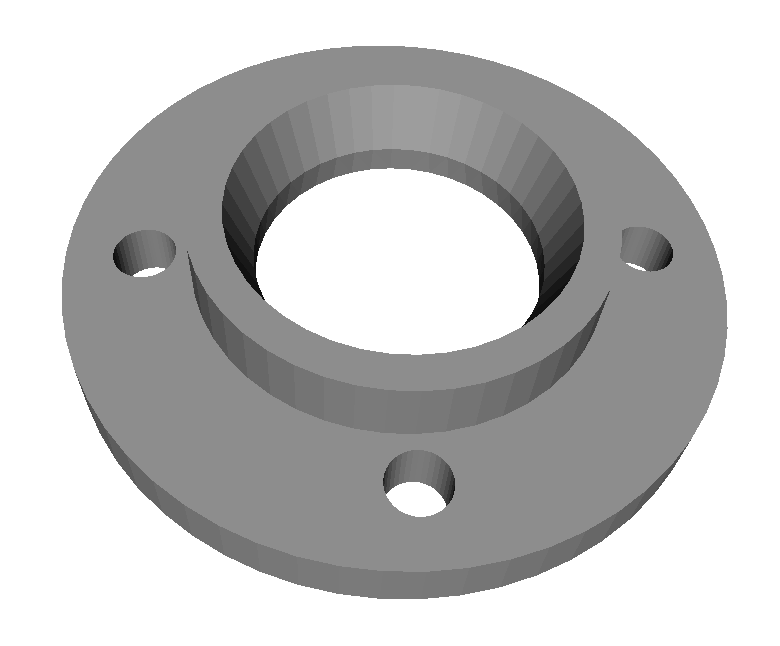
\includegraphics[width=1\linewidth]{./fig/eval/toshiba_flange1.png}
		\caption{Flange}
	\end{subfigure} \\ 
	\begin{subfigure}[b]{0.16\linewidth} \centering
		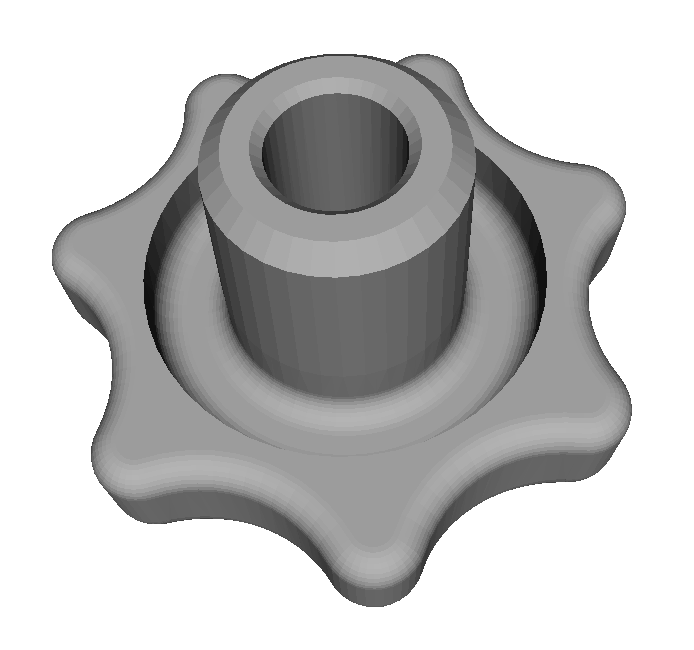
\includegraphics[width=1\linewidth]{./fig/eval/toshiba_knob1.png}
		\caption{Knob}
	\end{subfigure} 
	\begin{subfigure}[b]{0.16\linewidth} \centering
		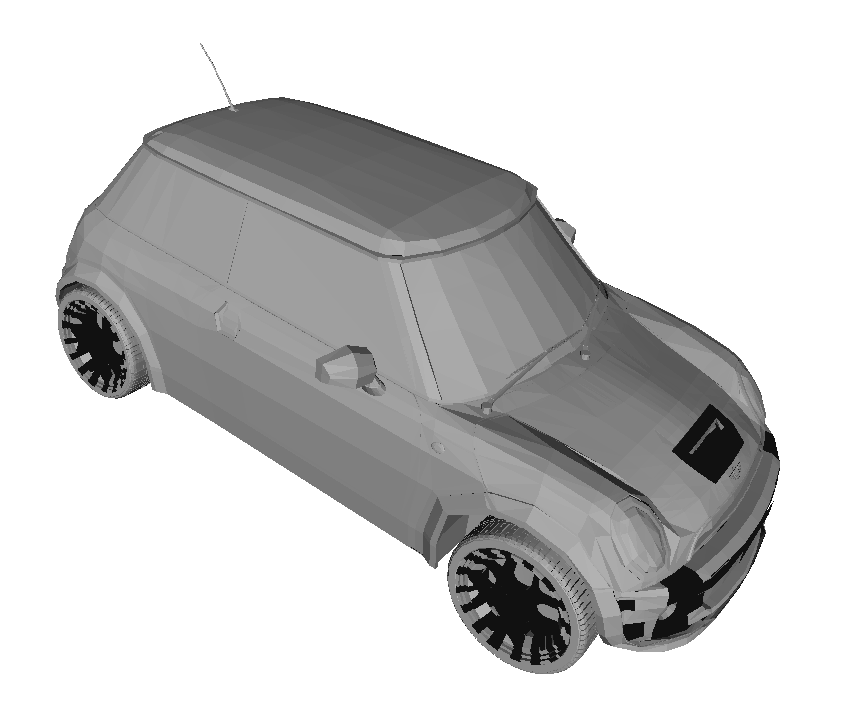
\includegraphics[width=1\linewidth]{./fig/eval/toshiba_mini1.png}
		\caption{Car}
	\end{subfigure}
	\begin{subfigure}[b]{0.16\linewidth} \centering
		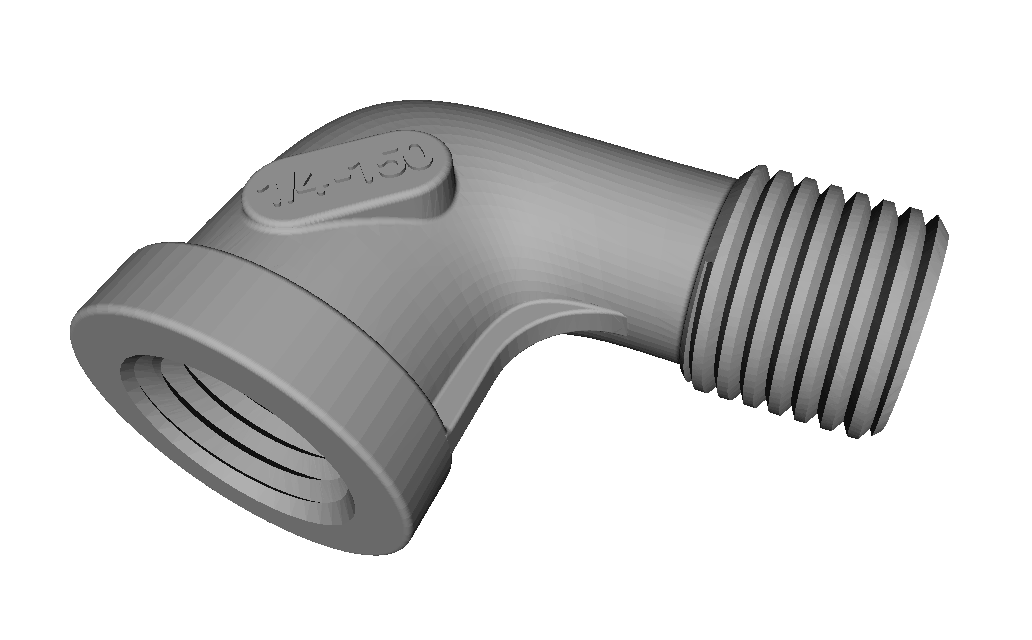
\includegraphics[width=1\linewidth]{./fig/eval/toshiba_pipe1.png}
		\caption{Pipe}
	\end{subfigure}
	\begin{subfigure}[b]{0.16\linewidth} \centering
		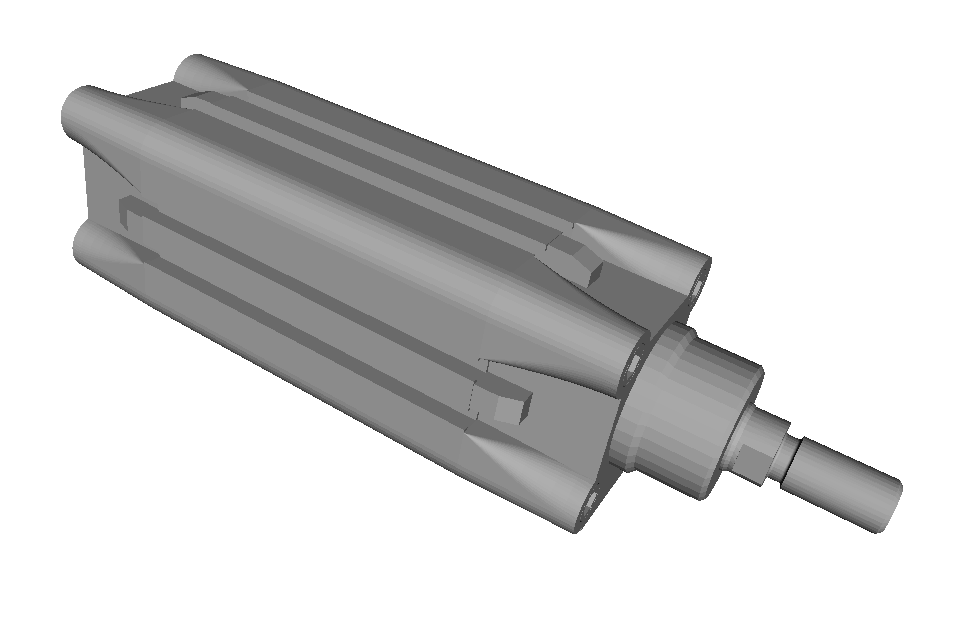
\includegraphics[width=1\linewidth]{./fig/eval/toshiba_piston1.png}
		\caption{Piston 1}
	\end{subfigure}
	\begin{subfigure}[b]{0.16\linewidth} \centering
		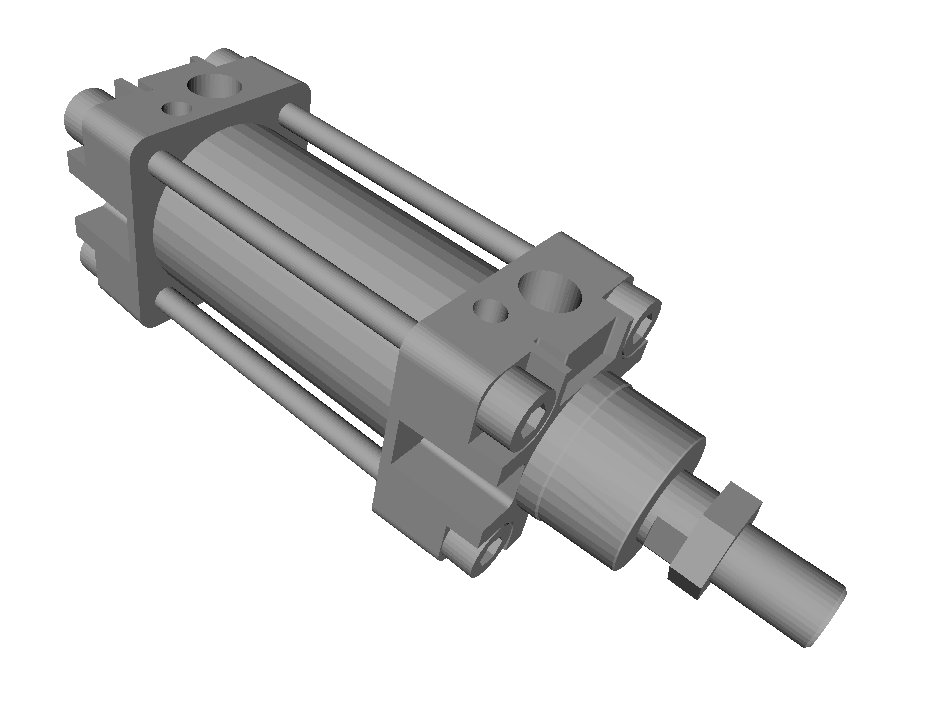
\includegraphics[width=1\linewidth]{./fig/eval/toshiba_piston2.png}
		\caption{Piston 2}
	\end{subfigure}
	\caption{\textbf{Sample CAD models of the \textbf{point cloud} dataset.}}
	\label{fig/reg/toshiba}
\end{figure}

The Toshiba CAD Model \textbf{point cloud} dataset \cite{Ltd.2011} was used for the 3D evaluation. It contains point clouds of 12 real objects acquired using multi-view stereo \cite{Vogiatzis2011}. Each object class contains 20 separate scans of a particular object, captured in a variety of poses. In this experiment, two shape classes, namely ``cog2'' and ``bearing1\_black'' were not included in the experiments because their shapes are too similar to other classes, \ie ``cog1'' and ``bearing1''. The ten classes of shapes included in the experiment are shown in figure \ref{fig/reg/toshiba} 

As point clouds are usually textureless, appearance features of the \textbf{Point cloud} dataset are described by the local shape around the interest points. 
The dataset includes a set of features per point cloud, each with position in scale, rotation and translation, as well as a $31$-dimensional descriptor, which are used for $\featshape_{\anyinstance\anyfeat}$ and $\featapp_{\anyinstance\anyfeat}$ respectively in the experiments. Furthermore, this dataset provides a ground truth pose for each object scan.
Similar to the \textbf{bike} dataset, the appearance descriptors were projected to a $10$-dimensional subspace using PCA.   
It has been found that more sophisticated features, \eg 3D shape context \cite{Frome2004}, gave similar performances with the default descriptor. Consequently, the simpler default descriptor was retained to demonstrate the effectiveness of the proposed model.


\subsection{Results: 2D images}

\subsubsection{Recognition}

The \textbf{bike} dataset was divided into two equal subsets, training was performed on one half while the remaining half was used in testing. The two subsets were swapped afterwards and final experimental results were combined.

Instances of the \textbf{bike} dataset were transformed randomly by both direct similarity and affine poses. For each type of pose, three levels of transformation were applied. Experimental results were compared with that of Fergus \etal \cite{Fergus2007}.   
Table \ref{tab/reg/regresult2d} summarises the experimental results. 
Performances figures are given by the ROC equal error rates for binary classification testing against the background dataset, such that a 50\% accuracy implies a random classifier. 
% Direct similarity and affine random transformation were applied to the training and testing instances. For each type of transformation, three levels of transformation were applied and compared with the results of Fergus \etal \cite{Fergus2007}. 
%We use the evaluation framework of \cite{Fergus2007}, randomly dividing the \textbf{bike} dataset into two equal subsets, training on one half and testing on the other and vice versa and summing the results. 
% The \textbf{bike} dataset is split randomly into two separate subsets. 
%A two-fold cross-validation is performed by training the model on one subset and testing on the other. 
%Two-fold cross validation is performed by randomly dividing the \textbf{bike} dataset into two equal subsets. 
%In order to evaluate the model's pose learning ability, we introduced three different levels of synthetic extra transformations. 
%Hence, there are effectively seven datasets with different amounts of pose variations. 

\begin{table}
	\centering
	\begin{tabular}{|c|cc|cc|c|}
		\hline 
		\textbf{Method} & \multicolumn{2}{|c|}{SAP (similarity)} & \multicolumn{2}{|c|}{SAP (affine)} & Fergus \etal \cite{Fergus2007} \\  
		\hline 
		\hline 
		$\numpart, \numparticle$ & 10, 5 & 6, 5 & 10, 5 & 6, 5 & 6, -- \\		
		\hline 
		\textbf{No pose} 		& \textbf{\color{blue}{95.500}} & 90.500 & 95.125 & 91.250 & 95.125 \\ 
		\hline 
		\textbf{Small pose} 	& \textbf{\color{blue}{94.625}} & 88.250 & 92.125 & 88.000 & 87.000 \\ 
		\textbf{Medium pose} 	& \textbf{\color{blue}{93.250}} & 87.250 & 83.125 & 78.250 & 60.000 \\ 
		\textbf{Large pose} 	& \textbf{\color{blue}{92.250}} & 85.750 & 75.750 & 70.500 & 52.000 \\ 
		\hline
		\textbf{Small pose} 	& \textbf{\color{blue}{94.625}} & 88.250 & 92.125 & 88.000 & 87.000 \\ 
		\textbf{Medium pose} 	& \textbf{\color{blue}{93.250}} & 87.250 & 83.125 & 78.250 & 60.000 \\ 
		\textbf{Large pose} 	& \textbf{\color{blue}{92.250}} & 85.750 & 75.750 & 70.500 & 52.000 \\ 
		\hline 
	\end{tabular}
	\caption{\textbf{2D classification results.} ROC equal error rates for binary classification of the \textbf{bike} dataset.}
	\label{tab/reg/regresult2d}
\end{table}

%Table \ref{tab/reg/regresult2d} shows the recognition results using the proposed model and the work of Fergus \etal~\cite{Fergus2007}. 
According to the experimental results, both approaches perform similarly when there is no or small pose variations. However, the performance of Fergus \etal \cite{Fergus2007}, which does not model pose as a variable, drops rapidly as the pose variation level increases. Under large pose variation, traditional constellation model \cite{Fergus2007} ceases working, leading to a random classification. 
By contrast, the SAP model with direct similarity pose maintains a high recognition rate under large direct similarity pose variations, while the affine model, for which feature rotation and scaling components are absent, performs slightly worse. 
Under affine transformations, the two types SAP model perform similarly, with a significant drop in performance under large pose variations. Since the computed features, \ie the rotated patches, are not affine-invariant, they are irreversibly distorted by shearing, leading to a weaker appearance model, especially $\partapp$.
The more flexible affine transformations might also over-fit the poses of some non-object testing instances, creating more false positives that affected the recognition accuracy. 

\begin{figure}[ht]
	\centering 
	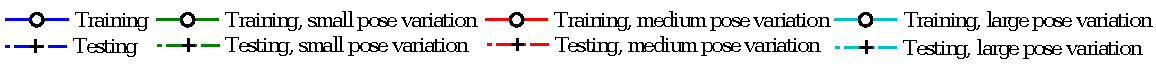
\includegraphics[width=1\linewidth]{fig/reg/reg2d_legend.pdf}
	\begin{subfigure}[b]{0.48\linewidth}
		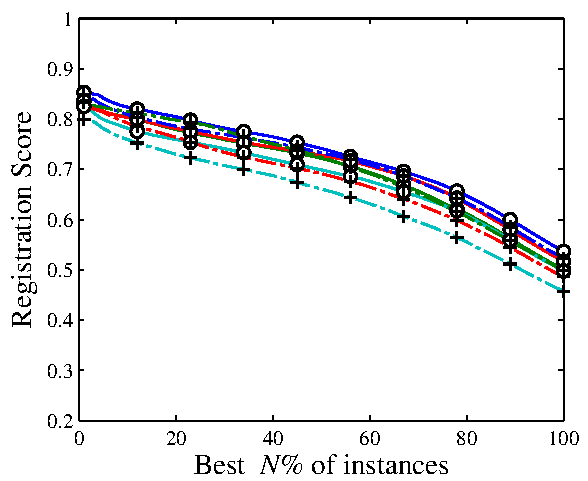
\includegraphics[width=\linewidth]{fig/reg/reg2d_simsim.pdf}
		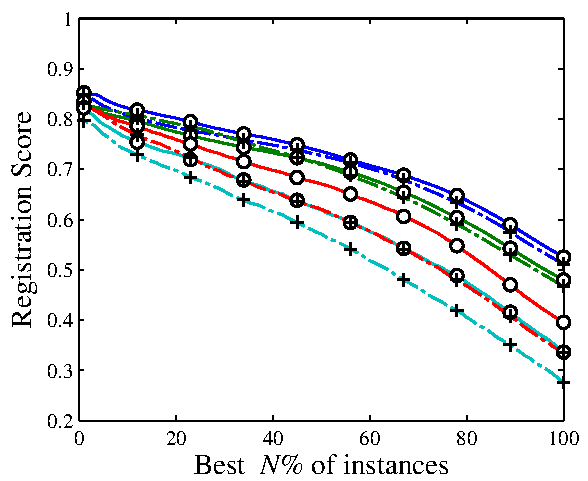
\includegraphics[width=\linewidth]{fig/reg/reg2d_simaff.pdf}
		\subcaption{SAP (pose model: similarity)}
	\end{subfigure}
	\begin{subfigure}[b]{0.48\linewidth}
		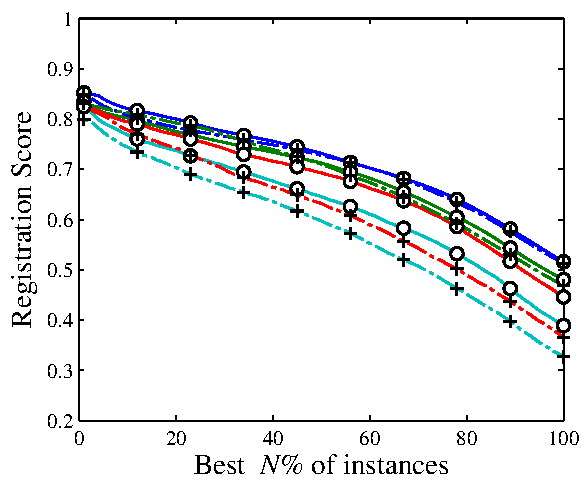
\includegraphics[width=\linewidth]{fig/reg/reg2d_affsim.pdf}
		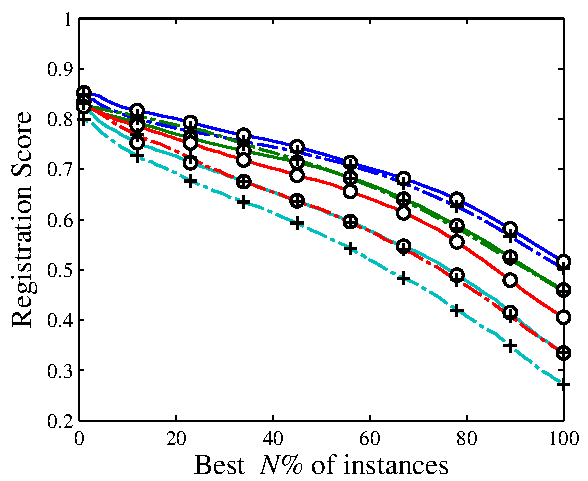
\includegraphics[width=\linewidth]{fig/reg/reg2d_affaff.pdf}
		\subcaption{SAP (pose model: affine)}
	\end{subfigure}
	\caption{\textbf{Registration scores for the \textbf{bike} dataset.} (a) similarity and (b) affine poses are evaluated using data with synthetic (left) similarity and (right) affine poses.}
	\label{fig/reg/regresult2d}
\end{figure}

\subsubsection{Registration} 
Since no ground truth pose is given in the original \textbf{bike} dataset, the registration capability of the SAP models was evaluated using hand-labelled pose information. 
%We create the registration dataset by selecting two hundred random object images from the \textbf{bike} dataset.
The registration score for the \textbf{bike} dataset was computed as follows.
Two hundred bikes images were randomly selected from the \textbf{bike} dataset; they were manually annotated the front and rear wheel centres, $\refptfront$ and $\refptrear$.
Similar to the recognition experiment, the dataset was divided into two halves for cross-validation. 
Reference points (wheel centres) of both the training and testing instances were projected into the canonical pose, using the learned poses. The training data points were then used to learn two normal distributions, $\NormDist(\cdot;\mu_\mathrm{front},\Sigma_\mathrm{front})$ and $\NormDist(\cdot;\mu_\mathrm{rear},\Sigma_\mathrm{rear})$, modelling the wheel centre locations, plus a uniform outlier distribution, $\UniformDist(\backgroundreg)$, using the EM algorithm. A registration score in the range $(0,1)$ was then computed for each training or test instance as
\begin{equation}
	\mathcal{S}_\mathrm{reg} = \frac{\NormDist(\pose\refptfront; \mu_\mathrm{front},\Sigma_\mathrm{front}) + \NormDist(\pose\refptrear; \mu_\mathrm{rear},\Sigma_\mathrm{rear})}{\NormDist(\pose\refptfront; \mu_\mathrm{front},\Sigma_\mathrm{front}) + \NormDist(\pose\refptrear; \mu_\mathrm{rear},\Sigma_\mathrm{rear}) + 2\UniformDist(\backgroundreg)}.
	\label{eqn/reg/reg2d_score}
\end{equation}
Figure \ref{fig/reg/regresult2d} plots the registration scores under different levels of pose variation, which corroborate the recognition results in terms of relative performance. 
Comparable training and test scores indicate that the learned model transfers well to unseen data. The similarity-pose SAP model performs better than its affine-pose variant. Similar to the recognition experiment, it is mainly due to the non-similarity distortion of appearance features, \eg shearing. 

\subsection{Results: 3D shapes}

\subsubsection{Recognition}
Following Pham \etal \cite{Pham2011}, leave-one-out cross validation scheme was used to measure multi-class recognition accuracy on the \textbf{point cloud} dataset. One instance was taken out from the dataset each time as a test shape, while the remaining $19$ instances were used to train the object recogniser. Ten classes from the dataset were evaluated, thus 200 separate models were trained for the experiments. The optimal operating point, \ie decision threshold, was adjusted from the training data to maintain a maximum false positive rate of $5\%$. 

\begin{figure}[ht]
	\centering
	\begin{subfigure}[t]{0.32\linewidth}
		\label{fig/reg/confusion_sap}
		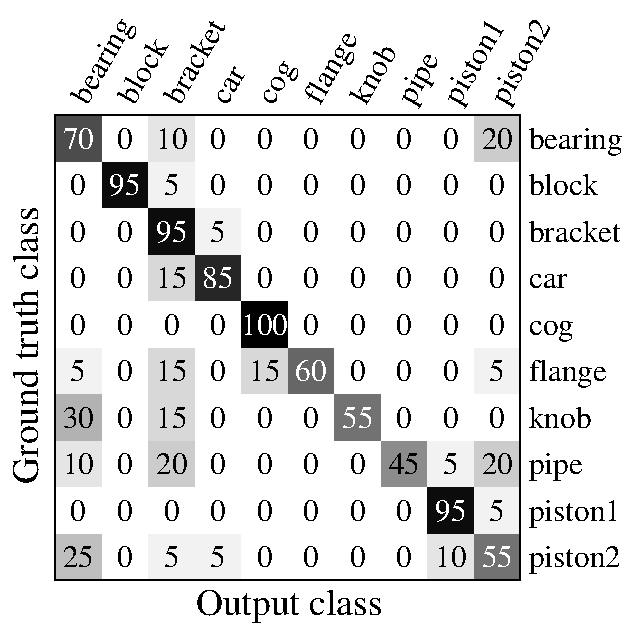
\includegraphics[width=1\linewidth]{fig/reg/confusion_sap.pdf}
		\subcaption{SAP}
	\end{subfigure}
	\begin{subfigure}[t]{0.32\linewidth}
		\label{fig/reg/confusion_meanshift}
		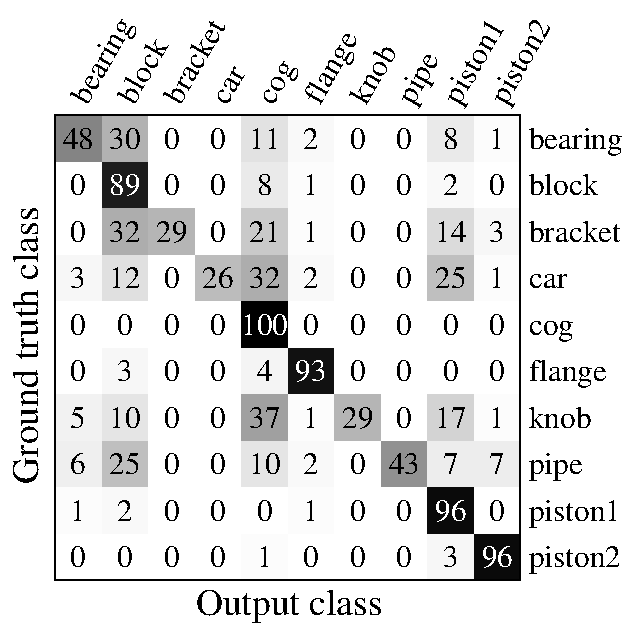
\includegraphics[width=1\linewidth]{fig/reg/confusion_meanshift.pdf}
		\subcaption{Meanshift \cite{Pham2011}}
	\end{subfigure}
	\begin{subfigure}[t]{0.32\linewidth}
		\label{fig/reg/confusion_intrinsic}
		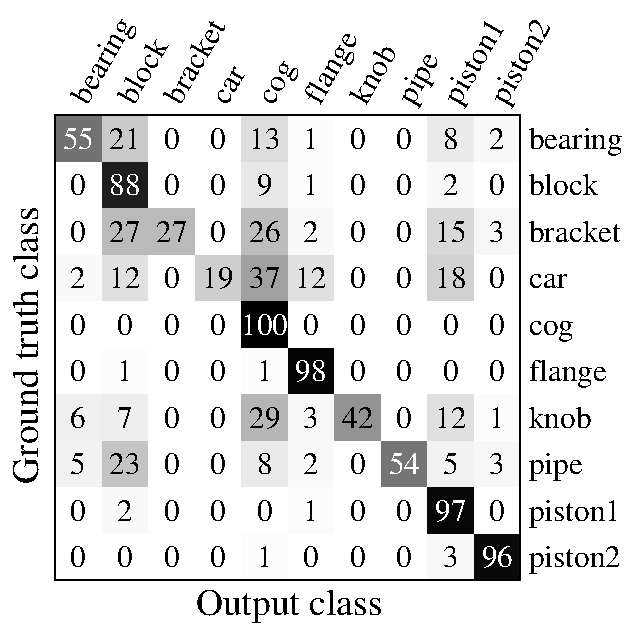
\includegraphics[width=1\linewidth]{fig/reg/confusion_intrinsic.pdf}
		\subcaption{Intrinsic Hough \cite{Woodford2013}}
	\end{subfigure}
	\begin{subfigure}[t]{0.32\linewidth}
		\label{fig/reg/confusion_minent}
		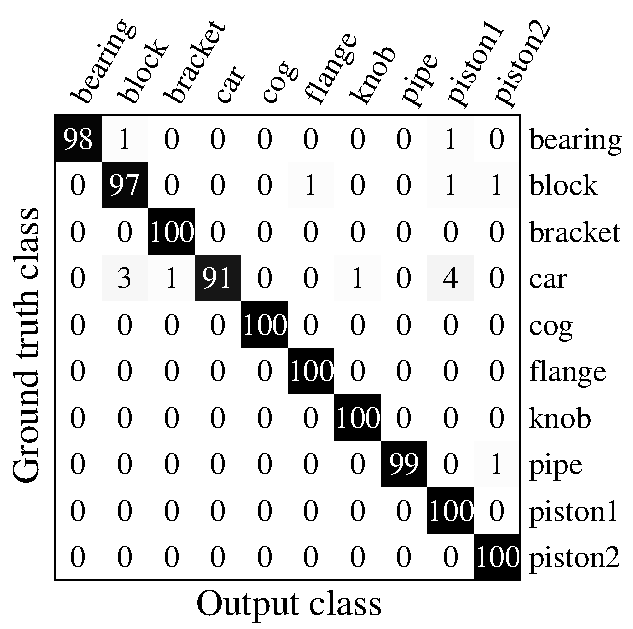
\includegraphics[width=1\linewidth]{fig/reg/confusion_minent.pdf}
		\subcaption{Minimum entropy Hough \cite{Woodford2013}}
	\end{subfigure}
	\begin{subfigure}[t]{0.32\linewidth}
		\label{fig/reg/confusion_blk}
		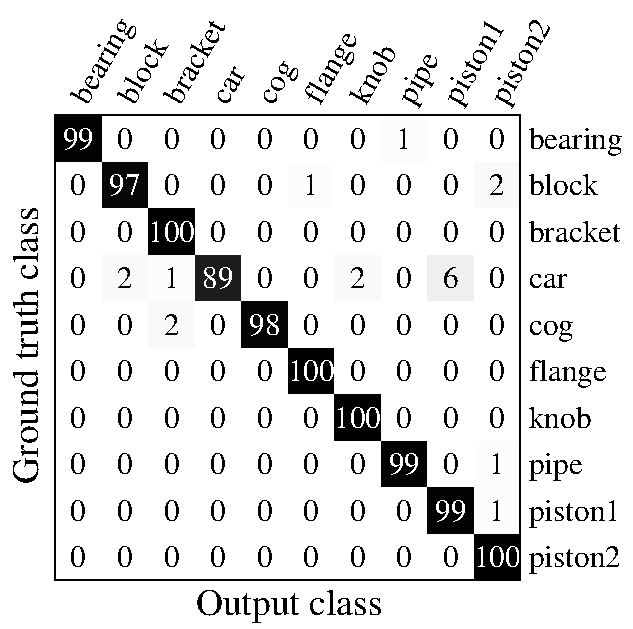
\includegraphics[width=1\linewidth]{fig/reg/confusion_blk.pdf}
		\subcaption{BLK \cite{Barinova2010}}
	\end{subfigure}
	\caption{\textbf{Confusion matrices.} From left to right: (a) our approach, (b) Mean shift, (c) Intrinsic Hough, (d) Minimum-entropy Hough and (e) BLK.}
	\label{fig/reg/recresult3d}
\end{figure}


%\begin{table}
%\centering
%{\footnotesize
%\begin{tabular}{|c|c|c|c|c|c|}
%\hline
%\textbf{Approach} & \emph{SAP} & Mean shift~\cite{Pham2011} & Intrinsic H.~\cite{Woodford2013} & Min.-ent. H.~\cite{Woodford2013} & BLK~\cite{Barinova2010} \\ 
%\hline
%\textbf{Avg. acc. (\%)} & 75.0 & 64.9 & 67.6 & 98.5 & 98.1 \\ 
%\hline
%\end{tabular}
%}
%\caption{The average object recognition accuracies.}
%\label{tab/reg/recresult3d}
%\end{table}


Figure \ref{fig/reg/recresult3d} shows the confusion matrices of the proposed SAP model and existing state-of-the-arts, using the direct similarity pose parameterisation. (Note that SAP model is a binary object class classifier, thus the rows of its confusion matrix do not sum to $100$.)
The weakly-supervised SAP model achieves satisfactory results of 75.5\% multi-class recognition accuracy, while the latest reported state-of-the-art accuracy, using ground truth pose, is 98.5\% \cite{Woodford2013}. However, in the experiments, all approaches except SAP require manually registered training data.    
%However, the combined multi-class classifier is biased towards some stronger classes, \eg \emph{bracket}, as shown in figure \ref{fig/reg/confusion_sap}.

\subsubsection{Registration} 
\label{sec/reg/reg}
Registration of the \textbf{point cloud} dataset was evaluated quantitatively using SRT distances \cite{Pham2011} between pairs of instances. Given the ground truth pose, $\pose_\mathrm{gt}$, of an instance, the learned pose relative to the ground truth object coordinate frame is $\tilde{\pose} = \pose_\mathrm{gt}\pose^{-1}$.  
The registration criterion of \cite{Pham2011} is employed in this experiment. A pair of instances are considered registered correctly when their $\tilde{\pose}$ are within $5\%$ in scale, $\pi/12$ in orientation and $10\%$ in relative translation.

\begin{figure}[ht]
	\centering
	\begin{subfigure}[b]{0.23\linewidth}
		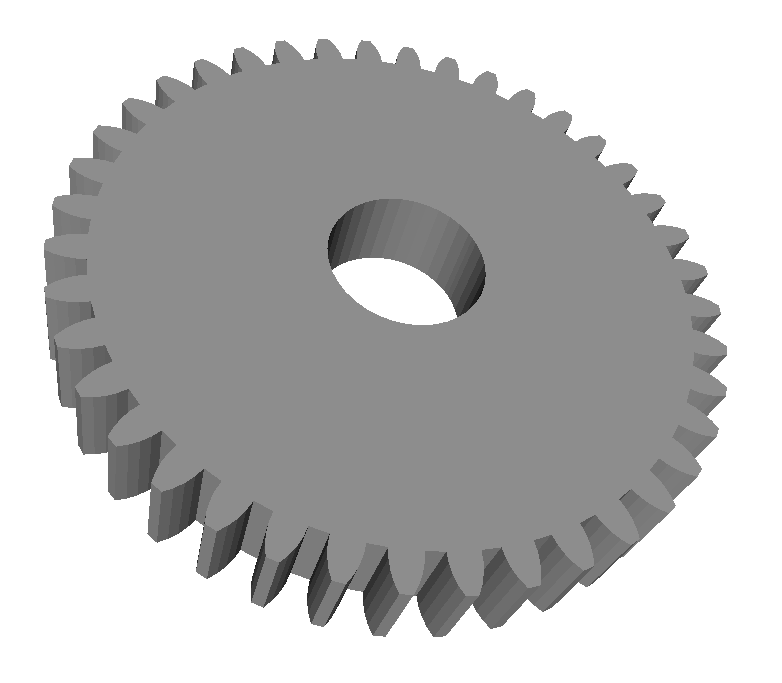
\includegraphics[width=\linewidth]{fig/reg/cog.png} \\
		
\includegraphics[width=\linewidth]{fig/reg/reg3Dtrain_cog.png} 
		\subcaption{Cog}
	\end{subfigure}
	\begin{subfigure}[b]{0.23\linewidth}
		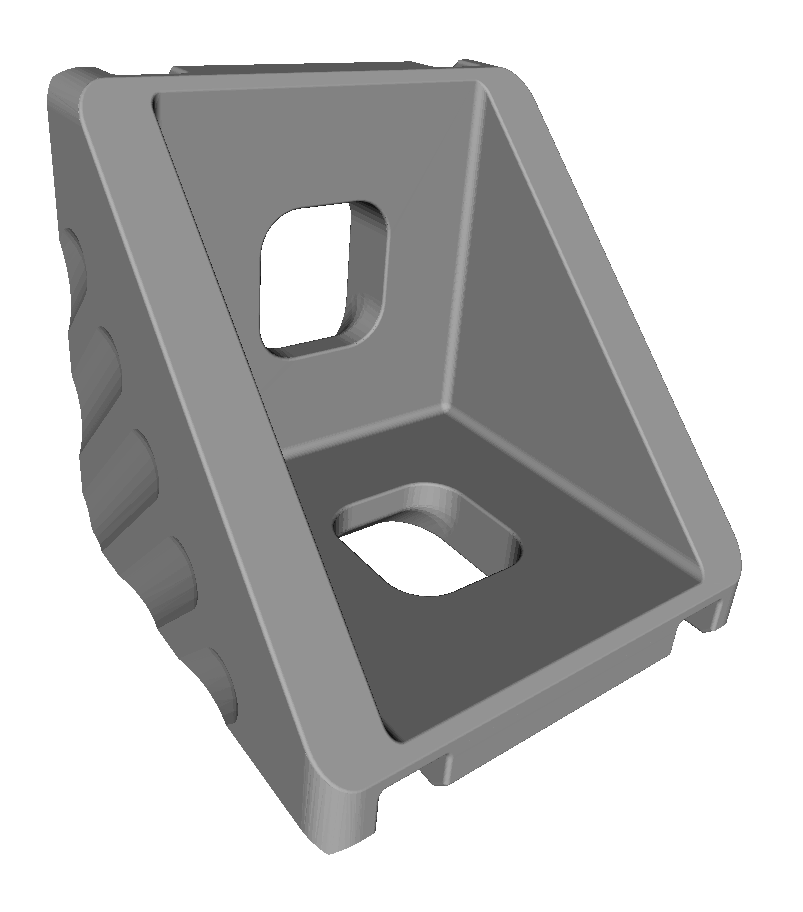
\includegraphics[width=\linewidth]{fig/reg/bracket.png} \\
		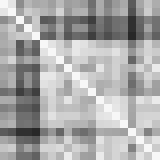
\includegraphics[width=\linewidth]{fig/reg/reg3Dtrain_bracket.png} 
		\subcaption{Bracket}
	\end{subfigure}
	\begin{subfigure}[b]{0.23\linewidth}
		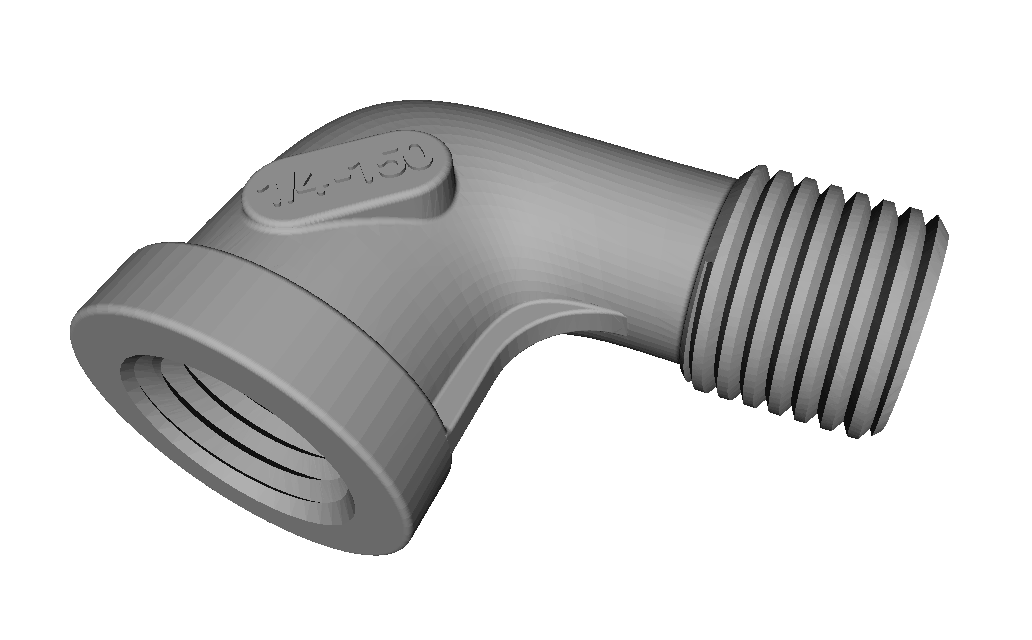
\includegraphics[width=\linewidth]{fig/reg/pipe.png} \\
		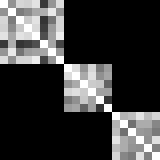
\includegraphics[width=\linewidth]{fig/reg/reg3Dtrain_pipe.png} 
		\subcaption{Pipe}
	\end{subfigure}
	\begin{subfigure}[b]{0.23\linewidth}
		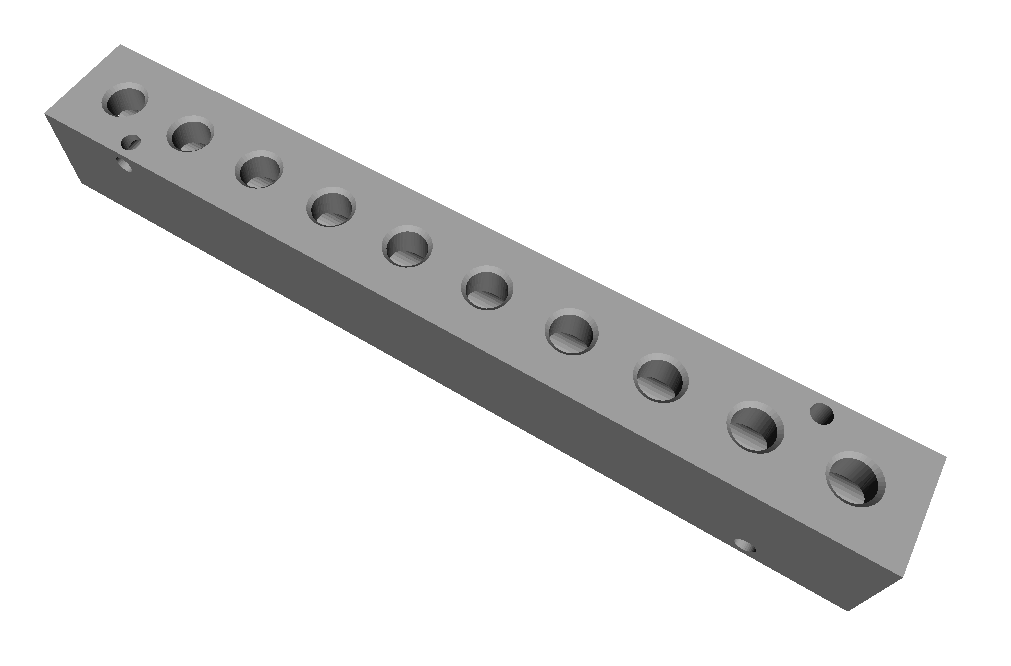
\includegraphics[width=\linewidth]{fig/reg/block.png} \\
		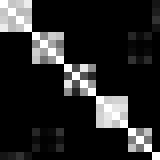
\includegraphics[width=\linewidth]{fig/reg/reg3Dtrain_block.png} 
		\subcaption{Block}
	\end{subfigure}
	\caption{\textbf{Distance matrices.} The values are visualised in $\exp(-\dist())$, where $\dist()$ is the SRT distance. Note that the bad registered classes, \eg \emph{block}, are clustered.}
	\label{fig/reg/reg_srtmatrices}
\end{figure}

\begin{figure}[ht] 
\centering
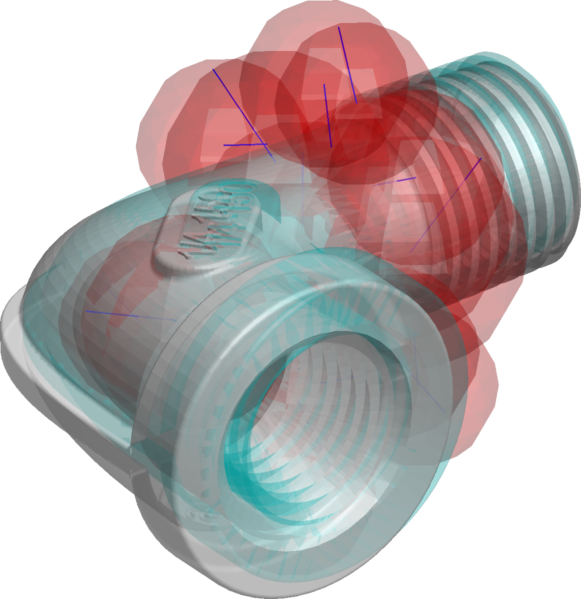
\includegraphics[width=0.19\linewidth]{fig/reg/shape01.png} \hspace{-1.5mm}
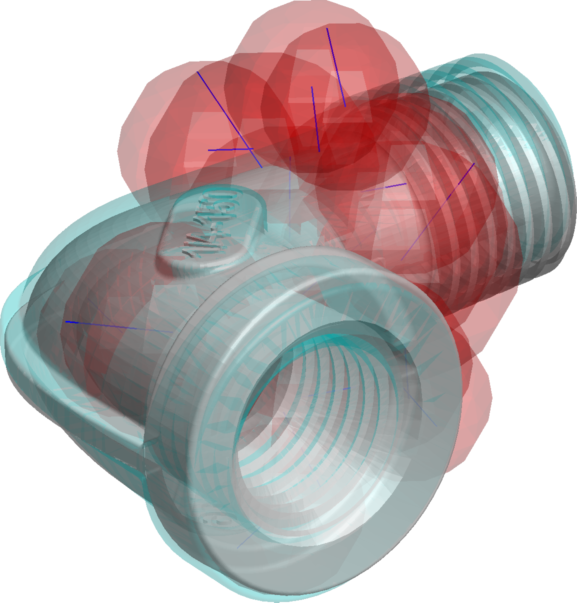
\includegraphics[width=0.19\linewidth]{fig/reg/shape02.png} \hspace{-1.5mm}
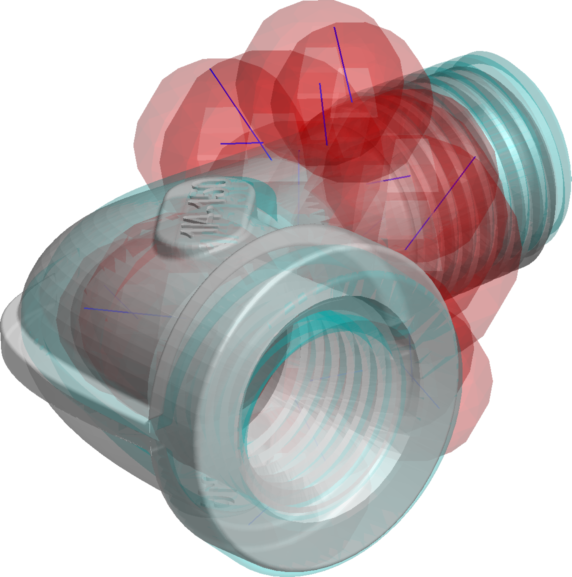
\includegraphics[width=0.19\linewidth]{fig/reg/shape03.png} \hspace{-1.5mm}
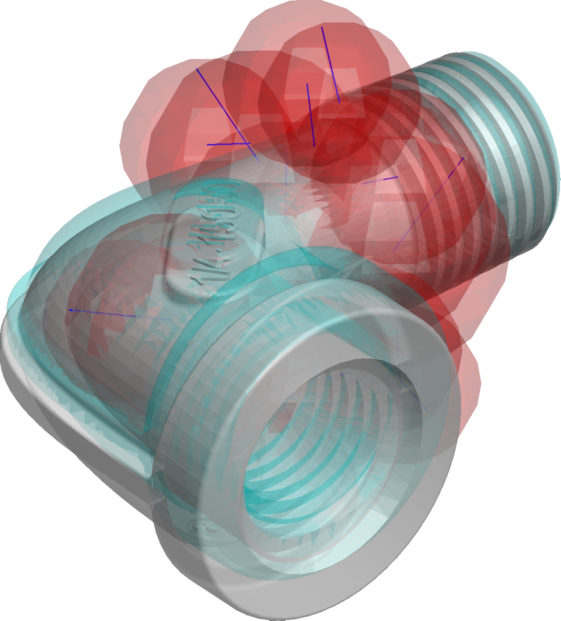
\includegraphics[width=0.19\linewidth]{fig/reg/shape04.png} \hspace{-1.5mm}
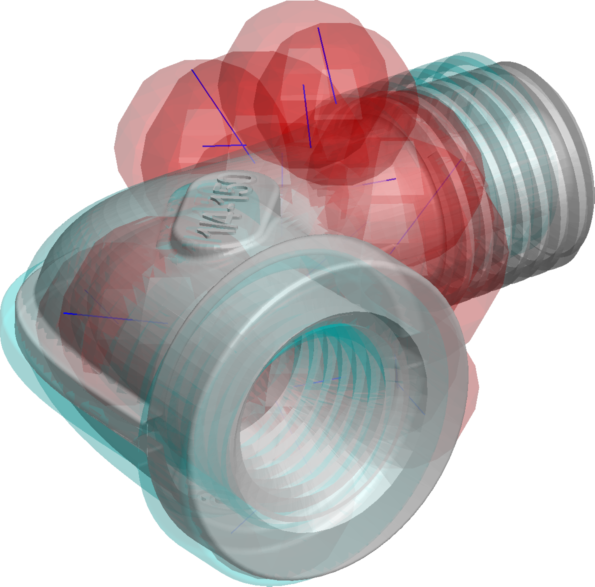
\includegraphics[width=0.19\linewidth]{fig/reg/shape05.png} \hspace{-1.5mm}
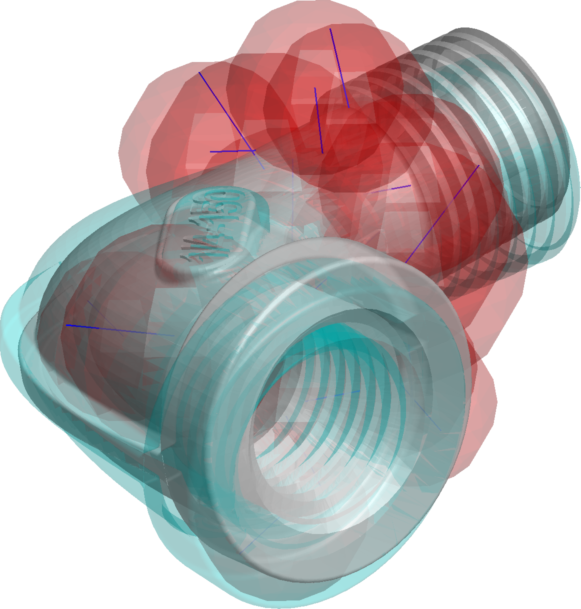
\includegraphics[width=0.19\linewidth]{fig/reg/shape06.png} \hspace{-1.5mm}
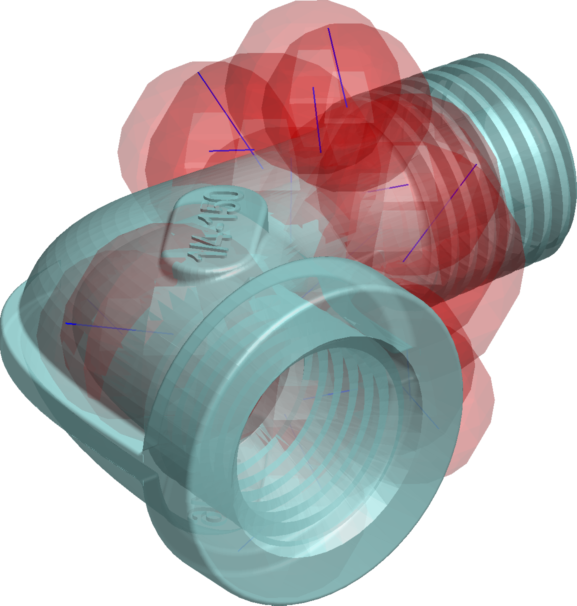
\includegraphics[width=0.19\linewidth]{fig/reg/shape07.png} \hspace{-1.5mm}
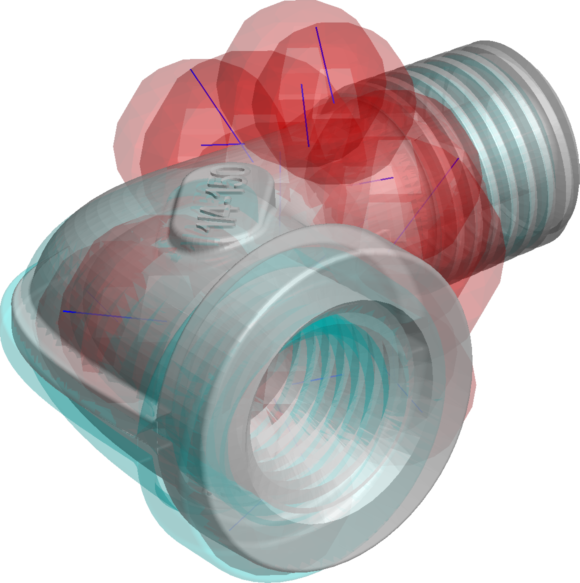
\includegraphics[width=0.19\linewidth]{fig/reg/shape08.png} \hspace{-1.5mm} 
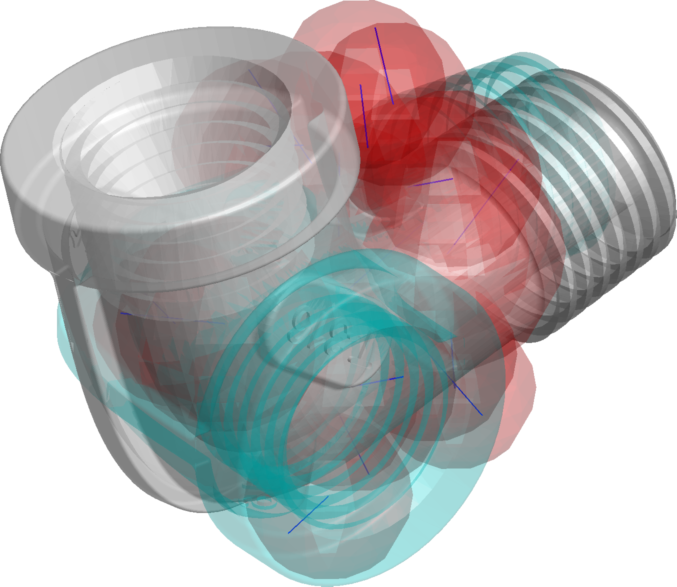
\includegraphics[width=0.19\linewidth]{fig/reg/shape09.png} \hspace{-1.5mm}
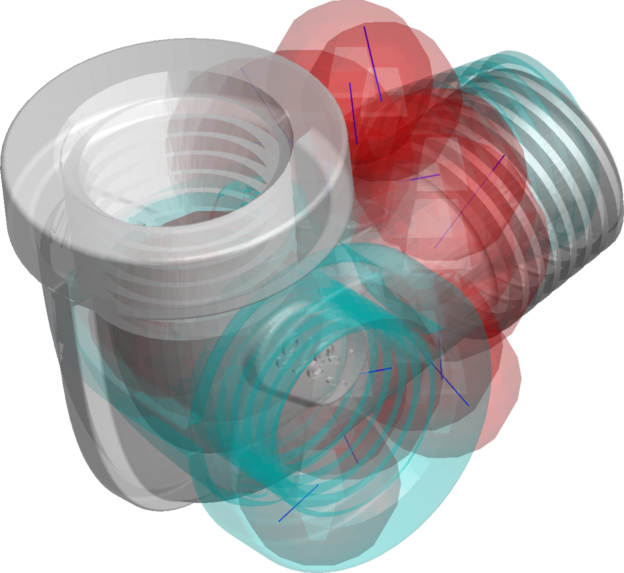
\includegraphics[width=0.19\linewidth]{fig/reg/shape10.png} \hspace{-1.5mm} \\ 
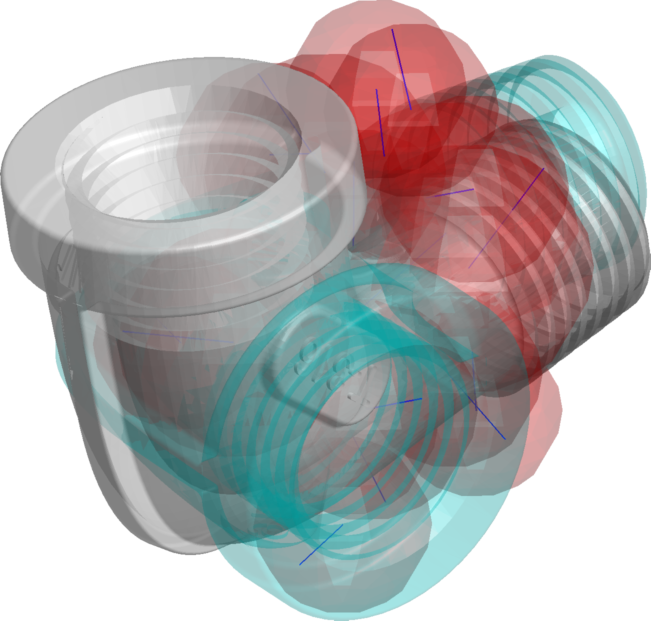
\includegraphics[width=0.19\linewidth]{fig/reg/shape11.png} \hspace{-1.5mm}
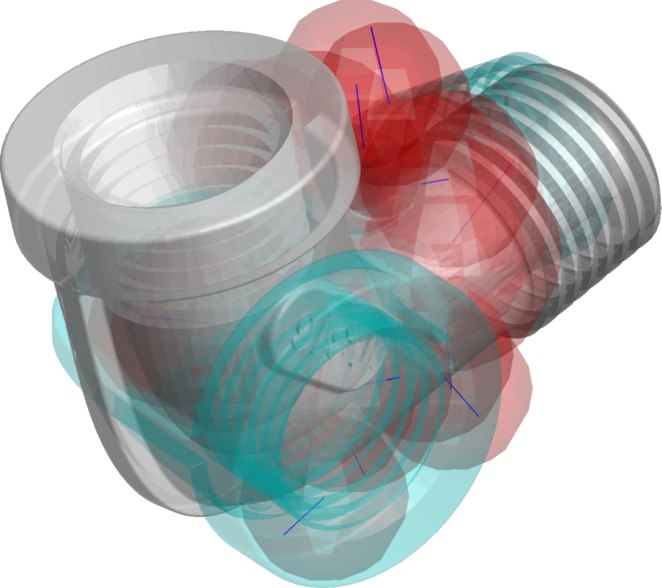
\includegraphics[width=0.19\linewidth]{fig/reg/shape12.png} \hspace{-1.5mm}
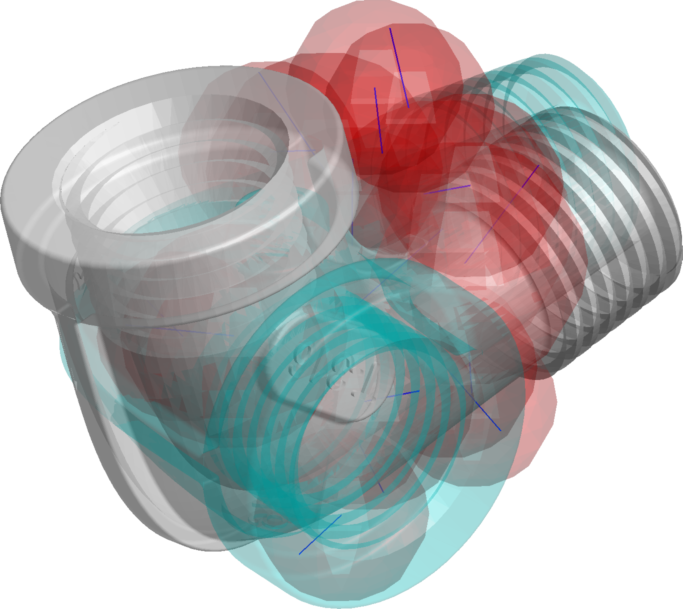
\includegraphics[width=0.19\linewidth]{fig/reg/shape13.png} \hspace{-1.5mm}
\includegraphics[width=0.19\linewidth]{fig/reg/shape14.png} \hspace{-1.5mm} 
\includegraphics[width=0.19\linewidth]{fig/reg/shape15.png} \hspace{-1.5mm}
\includegraphics[width=0.19\linewidth]{fig/reg/shape16.png} \hspace{-1.5mm}
\includegraphics[width=0.19\linewidth]{fig/reg/shape17.png} \hspace{-1.5mm}
\includegraphics[width=0.19\linewidth]{fig/reg/shape18.png} \hspace{-1.5mm}
\includegraphics[width=0.19\linewidth]{fig/reg/shape19.png} \hspace{-1.5mm}
\includegraphics[width=0.19\linewidth]{fig/reg/shape20.png} \vspace{2mm}
\caption{\textbf{3D registration results.} \emph{Grey}: Inferred poses of the 20 \emph{pipe} class training instances. \emph{Cyan spheres}: the learned \emph{canonical pose}. \emph{Red spheres}: The locations and scales of parts.}
\label{fig/reg/alignresult3d}
\end{figure}

\iffalse
\begin{figure}[ht]
	\centering 
	\includegraphics[width=0.4\linewidth]{fig/reg/confusion_sap.pdf}
	\caption{Confusion matrix of SAP model}
	\label{fig/reg/confusion_sap}
\end{figure}
\fi 

For evaluation of registration in training, every training instance was compared with each of the 20 instances, giving a $20 \times 20$ SRT distance matrix. Figure \ref{fig/reg/reg_srtmatrices} visualises these matrices for several classes in the \textbf{point cloud} dataset, demonstrating that for some classes, distinct pose clusters have been observed. Figure \ref{fig/reg/alignresult3d} indicates that these clusters form around a small number of distinct poses that the object was captured in, latching onto background features in this situation. 

Figure \ref{fig/reg/3dclusters} visualises the groups of distinct poses of the point clouds, showing that the clustering issue is originated from the raw point clouds captured. Initialising poses to the ground truth during learning still led to these clusters, hence it shows that initialisation is not related to the above pose clustering problem. Since the \textbf{bike} dataset contains images of different bikes on different backgrounds, it does not suffer from this issue.

%%%%%%%%%%%%%%%%% TESTING REGISTRATION
For evaluating the performance of 3D object recognition during testing, the $\tilde{\pose}$ of each test instance was compared to that of the training instance which gave the lowest Euclidean distance of its part-wise likelihood with that of the test instance. The per-class registration results are given in table \ref{tab/reg/regresult3d}, where they are compared with state-of-the-art results of a supervised, vote-based approach \cite{Woodford2013}, \ie ground truth pose data were given in training. Despite the SAP model having the handicap of not using ground truth pose, it obtains the highest score on half the classes.

\begin{figure}[ht]
	\centering
	\begin{subfigure}[b]{0.33\linewidth}
		\includegraphics[width=\linewidth]{fig/reg/cluster1.png}
		\subcaption{Scans 1--8}
	\end{subfigure}
	\begin{subfigure}[b]{0.32\linewidth}
		\includegraphics[width=\linewidth]{fig/reg/cluster2.png}
		\subcaption{Scans 9--14}
	\end{subfigure}
	\begin{subfigure}[b]{0.30\linewidth}
		\includegraphics[width=\linewidth]{fig/reg/cluster3.png}
		\subcaption{Scans 15--20}
	\end{subfigure}
	\caption{\textbf{Pose clusters in from data acquisition.} Raw data captured in three distinct poses for the \emph{pipe} class lead to the three pose clusters.}
	\label{fig/reg/3dclusters}
\end{figure}

\iffalse 
\begin{table}[t]
\centering
\begin{tabular}{|c|c|c|c|c|c|c|c|c|c|c|c|c|}
\hline
\multirow{2}{*}{\textbf{Method}} & \multicolumn{10}{|c|}{\textbf{Category}} & \multirow{2}{*}{\textbf{Average}} \\
\cline{2-11}
& \rotatebox{90}{{bearing}}& 
\rotatebox{90}{{block}}& 
\rotatebox{90}{{bracket}}& 
\rotatebox{90}{{car}}& 
\rotatebox{90}{{cog}}& 
\rotatebox{90}{{flange}}& 
\rotatebox{90}{{knob}}& 
\rotatebox{90}{{pipe}}& 
\rotatebox{90}{{piston1}} & 
\rotatebox{90}{{piston2}} & \\
\hline
SAP ($\numpart = 15, \numparticle = 10$)%\remarka
 & 50 & \textbf{35} & \textbf{100} & 75 & \textbf{100} & \textbf{60} & 65 & 25 & 45 & \textbf{95} & 65.0\\
\hline
Minimum entropy Hough \cite{Woodford2013} & \textbf{83} & 20 & 98 & \textbf{91} & \textbf{100} & 36 & \textbf{91} & \textbf{89} & \textbf{54} & 84 & \textbf{74.6}\\
\hline
\end{tabular}
\caption{\textbf{Object registration results for the \textbf{point cloud} dataset.}}
\label{tab/reg/regresult3d}
\end{table}
\fi 

\begin{table}[ht]
	\centering
	\begin{tabular}{|c|c|c|c|}
		\hline 	
		\multicolumn{2}{|c|}{\textbf{Method}} & SAP ($\numpart = 15, \numparticle = 10$) & Minimum entropy Hough \cite{Woodford2013} \\ \hline \hline 
		\multirow{10}{*}{\textbf{Shape}} & bearing & 50\% & \textbf{\color{blue}{83\%}} \\ \cline{2-4}  
		& block & \textbf{\color{blue}{35\%}} & 20\% \\ \cline{2-4} 
		& bracket & \textbf{\color{blue}{100\%}} & 98\% \\ \cline{2-4}
		& car & 75\% & \textbf{\color{blue}{91\%}} \\ \cline{2-4}
		& cog & \textbf{\color{blue}{100\%}} & \textbf{\color{blue}{100\%}} \\ \cline{2-4}
		& flange & \textbf{\color{blue}{60\%}} & 36\% \\ \cline{2-4}
		& knob & 65\% & \textbf{\color{blue}{91\%}} \\ \cline{2-4}
		& pipe & 25\% & \textbf{\color{blue}{89\%}} \\ \cline{2-4}
		& piston1 & 45\% & \textbf{\color{blue}{54\%}} \\ \cline{2-4}
		& piston2 & \textbf{\color{blue}{95\%}} & 84\% \\ \hline 
		\multicolumn{2}{|c|}{\textbf{Average}} & 65.0\% & \textbf{\color{blue}{74.6\%}} \\ \hline 
	\end{tabular}
	\caption{\textbf{Object registration results for the \textbf{point cloud} dataset.}}
	\label{tab/reg/regresult3d}
\end{table}

\section{Summary}
\label{sec/reg/conclusions}
% recap of our work

This chapter is concerned with the classification and pose estimation of 3D geometric shapes. 

Addressing the problem of learning a 3D shape recognition system from large-scale, un-annotated datasets, a generative shape, appearance and pose (SAP) model is presented. Different from traditional part-based model, the proposed SAP framework jointly learns a constellation model and the poses of training instances, additionally providing registration capability on top of recognition. The introduction of latent object pose in training greatly increases the parameter space, leading to a difficult optimisation problem for inference. However, such issue is solved by introducing a novel, particle-based optimisation scheme.  

%We have demonstrated not only that inferring pose 
The experimental results have demonstrated that inferring pose jointly with shape and appearance is feasible in practice. The proposed system performs only marginally worse than existing state-of-the-arts which use ground truth pose, and significantly improves on other approaches when ground truth pose is not known.  

% experiments

% what is so important? and future work?
%We hope that this work will lead to object recognition systems learned from large-scale, un-annotated datasets, including those which use only the estimated registrations from training to then learn a different type of model. We plan to extend this approach to learn a 3D constellation model of an object, along with 3D poses, from a series of 2D images.
